\documentclass[]{article}
\usepackage{lmodern}
\usepackage{amssymb,amsmath}
\usepackage{ifxetex,ifluatex}
\usepackage{fixltx2e} % provides \textsubscript
\ifnum 0\ifxetex 1\fi\ifluatex 1\fi=0 % if pdftex
  \usepackage[T1]{fontenc}
  \usepackage[utf8]{inputenc}
\else % if luatex or xelatex
  \ifxetex
    \usepackage{mathspec}
  \else
    \usepackage{fontspec}
  \fi
  \defaultfontfeatures{Ligatures=TeX,Scale=MatchLowercase}
\fi
% use upquote if available, for straight quotes in verbatim environments
\IfFileExists{upquote.sty}{\usepackage{upquote}}{}
% use microtype if available
\IfFileExists{microtype.sty}{%
\usepackage{microtype}
\UseMicrotypeSet[protrusion]{basicmath} % disable protrusion for tt fonts
}{}
\usepackage[margin=1in]{geometry}
\usepackage{hyperref}
\hypersetup{unicode=true,
            pdftitle={Modern Data Mining - HW 2},
            pdfauthor={Anirudh Bajaj; Esther Shin; Matt LeBaron},
            pdfborder={0 0 0},
            breaklinks=true}
\urlstyle{same}  % don't use monospace font for urls
\usepackage{color}
\usepackage{fancyvrb}
\newcommand{\VerbBar}{|}
\newcommand{\VERB}{\Verb[commandchars=\\\{\}]}
\DefineVerbatimEnvironment{Highlighting}{Verbatim}{commandchars=\\\{\}}
% Add ',fontsize=\small' for more characters per line
\usepackage{framed}
\definecolor{shadecolor}{RGB}{248,248,248}
\newenvironment{Shaded}{\begin{snugshade}}{\end{snugshade}}
\newcommand{\KeywordTok}[1]{\textcolor[rgb]{0.13,0.29,0.53}{\textbf{#1}}}
\newcommand{\DataTypeTok}[1]{\textcolor[rgb]{0.13,0.29,0.53}{#1}}
\newcommand{\DecValTok}[1]{\textcolor[rgb]{0.00,0.00,0.81}{#1}}
\newcommand{\BaseNTok}[1]{\textcolor[rgb]{0.00,0.00,0.81}{#1}}
\newcommand{\FloatTok}[1]{\textcolor[rgb]{0.00,0.00,0.81}{#1}}
\newcommand{\ConstantTok}[1]{\textcolor[rgb]{0.00,0.00,0.00}{#1}}
\newcommand{\CharTok}[1]{\textcolor[rgb]{0.31,0.60,0.02}{#1}}
\newcommand{\SpecialCharTok}[1]{\textcolor[rgb]{0.00,0.00,0.00}{#1}}
\newcommand{\StringTok}[1]{\textcolor[rgb]{0.31,0.60,0.02}{#1}}
\newcommand{\VerbatimStringTok}[1]{\textcolor[rgb]{0.31,0.60,0.02}{#1}}
\newcommand{\SpecialStringTok}[1]{\textcolor[rgb]{0.31,0.60,0.02}{#1}}
\newcommand{\ImportTok}[1]{#1}
\newcommand{\CommentTok}[1]{\textcolor[rgb]{0.56,0.35,0.01}{\textit{#1}}}
\newcommand{\DocumentationTok}[1]{\textcolor[rgb]{0.56,0.35,0.01}{\textbf{\textit{#1}}}}
\newcommand{\AnnotationTok}[1]{\textcolor[rgb]{0.56,0.35,0.01}{\textbf{\textit{#1}}}}
\newcommand{\CommentVarTok}[1]{\textcolor[rgb]{0.56,0.35,0.01}{\textbf{\textit{#1}}}}
\newcommand{\OtherTok}[1]{\textcolor[rgb]{0.56,0.35,0.01}{#1}}
\newcommand{\FunctionTok}[1]{\textcolor[rgb]{0.00,0.00,0.00}{#1}}
\newcommand{\VariableTok}[1]{\textcolor[rgb]{0.00,0.00,0.00}{#1}}
\newcommand{\ControlFlowTok}[1]{\textcolor[rgb]{0.13,0.29,0.53}{\textbf{#1}}}
\newcommand{\OperatorTok}[1]{\textcolor[rgb]{0.81,0.36,0.00}{\textbf{#1}}}
\newcommand{\BuiltInTok}[1]{#1}
\newcommand{\ExtensionTok}[1]{#1}
\newcommand{\PreprocessorTok}[1]{\textcolor[rgb]{0.56,0.35,0.01}{\textit{#1}}}
\newcommand{\AttributeTok}[1]{\textcolor[rgb]{0.77,0.63,0.00}{#1}}
\newcommand{\RegionMarkerTok}[1]{#1}
\newcommand{\InformationTok}[1]{\textcolor[rgb]{0.56,0.35,0.01}{\textbf{\textit{#1}}}}
\newcommand{\WarningTok}[1]{\textcolor[rgb]{0.56,0.35,0.01}{\textbf{\textit{#1}}}}
\newcommand{\AlertTok}[1]{\textcolor[rgb]{0.94,0.16,0.16}{#1}}
\newcommand{\ErrorTok}[1]{\textcolor[rgb]{0.64,0.00,0.00}{\textbf{#1}}}
\newcommand{\NormalTok}[1]{#1}
\usepackage{graphicx,grffile}
\makeatletter
\def\maxwidth{\ifdim\Gin@nat@width>\linewidth\linewidth\else\Gin@nat@width\fi}
\def\maxheight{\ifdim\Gin@nat@height>\textheight\textheight\else\Gin@nat@height\fi}
\makeatother
% Scale images if necessary, so that they will not overflow the page
% margins by default, and it is still possible to overwrite the defaults
% using explicit options in \includegraphics[width, height, ...]{}
\setkeys{Gin}{width=\maxwidth,height=\maxheight,keepaspectratio}
\IfFileExists{parskip.sty}{%
\usepackage{parskip}
}{% else
\setlength{\parindent}{0pt}
\setlength{\parskip}{6pt plus 2pt minus 1pt}
}
\setlength{\emergencystretch}{3em}  % prevent overfull lines
\providecommand{\tightlist}{%
  \setlength{\itemsep}{0pt}\setlength{\parskip}{0pt}}
\setcounter{secnumdepth}{0}
% Redefines (sub)paragraphs to behave more like sections
\ifx\paragraph\undefined\else
\let\oldparagraph\paragraph
\renewcommand{\paragraph}[1]{\oldparagraph{#1}\mbox{}}
\fi
\ifx\subparagraph\undefined\else
\let\oldsubparagraph\subparagraph
\renewcommand{\subparagraph}[1]{\oldsubparagraph{#1}\mbox{}}
\fi

%%% Use protect on footnotes to avoid problems with footnotes in titles
\let\rmarkdownfootnote\footnote%
\def\footnote{\protect\rmarkdownfootnote}

%%% Change title format to be more compact
\usepackage{titling}

% Create subtitle command for use in maketitle
\newcommand{\subtitle}[1]{
  \posttitle{
    \begin{center}\large#1\end{center}
    }
}

\setlength{\droptitle}{-2em}

  \title{Modern Data Mining - HW 2}
    \pretitle{\vspace{\droptitle}\centering\huge}
  \posttitle{\par}
    \author{Anirudh Bajaj \\ Esther Shin \\ Matt LeBaron}
    \preauthor{\centering\large\emph}
  \postauthor{\par}
    \date{}
    \predate{}\postdate{}
  

\begin{document}
\maketitle

\subsection{Overview / Instructions}\label{overview-instructions}

This is homework \#2 of STAT 471/571/701. It will be \textbf{due on Oct
10, 2018 by 11:59 PM} on Canvas. You can directly edit this file to add
your answers. Submit the Rmd file, a PDF or word or HTML version with
only 1 submission per HW team.

\subsection{Problem 0}\label{problem-0}

Review the code and concepts covered during lecture: multiple
regression, model selection and penalized regression through elastic
net.

\subsection{Problem 1}\label{problem-1}

Do ISLR, page 262, problem 8 only part (a) to (d) and write up the
answer here. This question is designed to help us understanding model
selections through simulations. (e) Describe as accurate as possible
what Cp and BIC are estimating?

\begin{enumerate}
\def\labelenumi{(\alph{enumi})}
\item
\end{enumerate}

\begin{Shaded}
\begin{Highlighting}[]
\CommentTok{# Use rnorm() to generate a predictor X of length n = 100, and a noise vector of length n = 100}
\NormalTok{x <-}\StringTok{ }\KeywordTok{rnorm}\NormalTok{(}\DecValTok{100}\NormalTok{)}
\NormalTok{noise <-}\StringTok{ }\KeywordTok{rnorm}\NormalTok{(}\DecValTok{100}\NormalTok{)}
\end{Highlighting}
\end{Shaded}

\begin{enumerate}
\def\labelenumi{(\alph{enumi})}
\setcounter{enumi}{1}
\item
\end{enumerate}

\begin{Shaded}
\begin{Highlighting}[]
\CommentTok{# Generate a response vector Y of length n = 100 according to the model}
\NormalTok{y <-}\StringTok{ }\DecValTok{1} \OperatorTok{+}\StringTok{ }\DecValTok{2}\OperatorTok{*}\NormalTok{x }\OperatorTok{+}\StringTok{ }\DecValTok{3}\OperatorTok{*}\NormalTok{x}\OperatorTok{^}\DecValTok{2} \OperatorTok{+}\StringTok{ }\DecValTok{4}\OperatorTok{*}\NormalTok{x}\OperatorTok{^}\DecValTok{3} \OperatorTok{+}\StringTok{ }\NormalTok{noise}
\end{Highlighting}
\end{Shaded}

\begin{enumerate}
\def\labelenumi{(\alph{enumi})}
\setcounter{enumi}{2}
\item
\end{enumerate}

\begin{Shaded}
\begin{Highlighting}[]
\CommentTok{# Create the predictors x^2 through x^10}
\NormalTok{x2 <-}\StringTok{ }\NormalTok{x}\OperatorTok{^}\DecValTok{2}
\NormalTok{x3 <-}\StringTok{ }\NormalTok{x}\OperatorTok{^}\DecValTok{3}
\NormalTok{x4 <-}\StringTok{ }\NormalTok{x}\OperatorTok{^}\DecValTok{4}
\NormalTok{x5 <-}\StringTok{ }\NormalTok{x}\OperatorTok{^}\DecValTok{5}
\NormalTok{x6 <-}\StringTok{ }\NormalTok{x}\OperatorTok{^}\DecValTok{6}
\NormalTok{x7 <-}\StringTok{ }\NormalTok{x}\OperatorTok{^}\DecValTok{7}
\NormalTok{x8 <-}\StringTok{ }\NormalTok{x}\OperatorTok{^}\DecValTok{8}
\NormalTok{x9 <-}\StringTok{ }\NormalTok{x}\OperatorTok{^}\DecValTok{9}
\NormalTok{x10 <-}\StringTok{ }\NormalTok{x}\OperatorTok{^}\DecValTok{10}

\CommentTok{# Use the regsubsets() function to perform best subset selection}
\NormalTok{new_data <-}\StringTok{ }\KeywordTok{data.frame}\NormalTok{(x,x2,x3,x4,x5,x6,x7,x8,x9,x10,noise,y)}
\NormalTok{new_subset <-}\StringTok{ }\KeywordTok{regsubsets}\NormalTok{(y }\OperatorTok{~}\StringTok{ }\NormalTok{x}\OperatorTok{+}\NormalTok{x2}\OperatorTok{+}\NormalTok{x3}\OperatorTok{+}\NormalTok{x4}\OperatorTok{+}\NormalTok{x5}\OperatorTok{+}\NormalTok{x6}\OperatorTok{+}\NormalTok{x7}\OperatorTok{+}\NormalTok{x8}\OperatorTok{+}\NormalTok{x9}\OperatorTok{+}\NormalTok{x10,}\DataTypeTok{data =}\NormalTok{ new_data, }\DataTypeTok{nvmax =} \DecValTok{10}\NormalTok{)}
\NormalTok{new_summary <-}\StringTok{ }\KeywordTok{summary}\NormalTok{(new_subset)}
\NormalTok{new_summary}\OperatorTok{$}\NormalTok{which}
\end{Highlighting}
\end{Shaded}

\begin{verbatim}
##    (Intercept)     x    x2   x3    x4    x5    x6    x7    x8    x9   x10
## 1         TRUE FALSE FALSE TRUE FALSE FALSE FALSE FALSE FALSE FALSE FALSE
## 2         TRUE FALSE  TRUE TRUE FALSE FALSE FALSE FALSE FALSE FALSE FALSE
## 3         TRUE  TRUE  TRUE TRUE FALSE FALSE FALSE FALSE FALSE FALSE FALSE
## 4         TRUE  TRUE  TRUE TRUE FALSE FALSE FALSE FALSE FALSE  TRUE FALSE
## 5         TRUE  TRUE  TRUE TRUE FALSE FALSE FALSE FALSE  TRUE FALSE  TRUE
## 6         TRUE  TRUE  TRUE TRUE FALSE FALSE  TRUE FALSE FALSE  TRUE  TRUE
## 7         TRUE  TRUE  TRUE TRUE  TRUE FALSE  TRUE FALSE  TRUE  TRUE FALSE
## 8         TRUE  TRUE  TRUE TRUE  TRUE  TRUE  TRUE  TRUE  TRUE FALSE FALSE
## 9         TRUE  TRUE  TRUE TRUE  TRUE  TRUE  TRUE  TRUE  TRUE FALSE  TRUE
## 10        TRUE  TRUE  TRUE TRUE  TRUE  TRUE  TRUE  TRUE  TRUE  TRUE  TRUE
\end{verbatim}

\begin{Shaded}
\begin{Highlighting}[]
\KeywordTok{data.frame}\NormalTok{(}\DataTypeTok{variables=}\NormalTok{(}\DecValTok{1}\OperatorTok{:}\KeywordTok{length}\NormalTok{(new_summary}\OperatorTok{$}\NormalTok{rsq)), }\DataTypeTok{r_squared=}\NormalTok{new_summary}\OperatorTok{$}\NormalTok{rsq)}
\end{Highlighting}
\end{Shaded}

\begin{verbatim}
##    variables r_squared
## 1          1 0.9415944
## 2          2 0.9922962
## 3          3 0.9970612
## 4          4 0.9970839
## 5          5 0.9972668
## 6          6 0.9973422
## 7          7 0.9973453
## 8          8 0.9973470
## 9          9 0.9973471
## 10        10 0.9973497
\end{verbatim}

\begin{Shaded}
\begin{Highlighting}[]
\CommentTok{# What is the best model obtained?}
\KeywordTok{data.frame}\NormalTok{(}\DataTypeTok{variables =}\NormalTok{ (}\DecValTok{1}\OperatorTok{:}\KeywordTok{length}\NormalTok{(new_summary}\OperatorTok{$}\NormalTok{rsq)),}
           \DataTypeTok{r_squared =}\NormalTok{ new_summary}\OperatorTok{$}\NormalTok{rsq,}
           \DataTypeTok{rss =}\NormalTok{ new_summary}\OperatorTok{$}\NormalTok{rss,}
           \DataTypeTok{bic =}\NormalTok{ new_summary}\OperatorTok{$}\NormalTok{bic,}
           \DataTypeTok{cp =}\NormalTok{ new_summary}\OperatorTok{$}\NormalTok{cp)}
\end{Highlighting}
\end{Shaded}

\begin{verbatim}
##    variables r_squared        rss       bic          cp
## 1          1 0.9415944 1521.06495 -274.8240 1865.319437
## 2          2 0.9922962  200.63206 -472.7882  164.702662
## 3          3 0.9970612   76.53679 -564.5531    6.689472
## 4          4 0.9970839   75.94426 -560.7252    7.925437
## 5          5 0.9972668   71.18062 -562.5979    3.783013
## 6          6 0.9973422   69.21825 -560.7883    3.252668
## 7          7 0.9973453   69.13604 -556.3020    5.146664
## 8          8 0.9973470   69.09373 -551.7581    7.092097
## 9          9 0.9973471   69.09046 -547.1576    9.087887
## 10        10 0.9973497   69.02230 -542.6511   11.000000
\end{verbatim}

The best model obtained has three variables: x, x2, and x3. This makes
sense because these three variables were used to generate Y in the first
place, so they should be most predictive, although they aren't perfect
because we added in noise as well.

\begin{Shaded}
\begin{Highlighting}[]
\CommentTok{# Comparing the plots for Cp, bic, and r2}
\KeywordTok{plot}\NormalTok{(new_summary}\OperatorTok{$}\NormalTok{cp, }\DataTypeTok{xlab=}\StringTok{"Number of predictors"}\NormalTok{, }
     \DataTypeTok{ylab=}\StringTok{"cp"}\NormalTok{, }\DataTypeTok{col=}\StringTok{"red"}\NormalTok{, }\DataTypeTok{type=}\StringTok{"p"}\NormalTok{, }\DataTypeTok{pch=}\DecValTok{16}\NormalTok{)}
\end{Highlighting}
\end{Shaded}

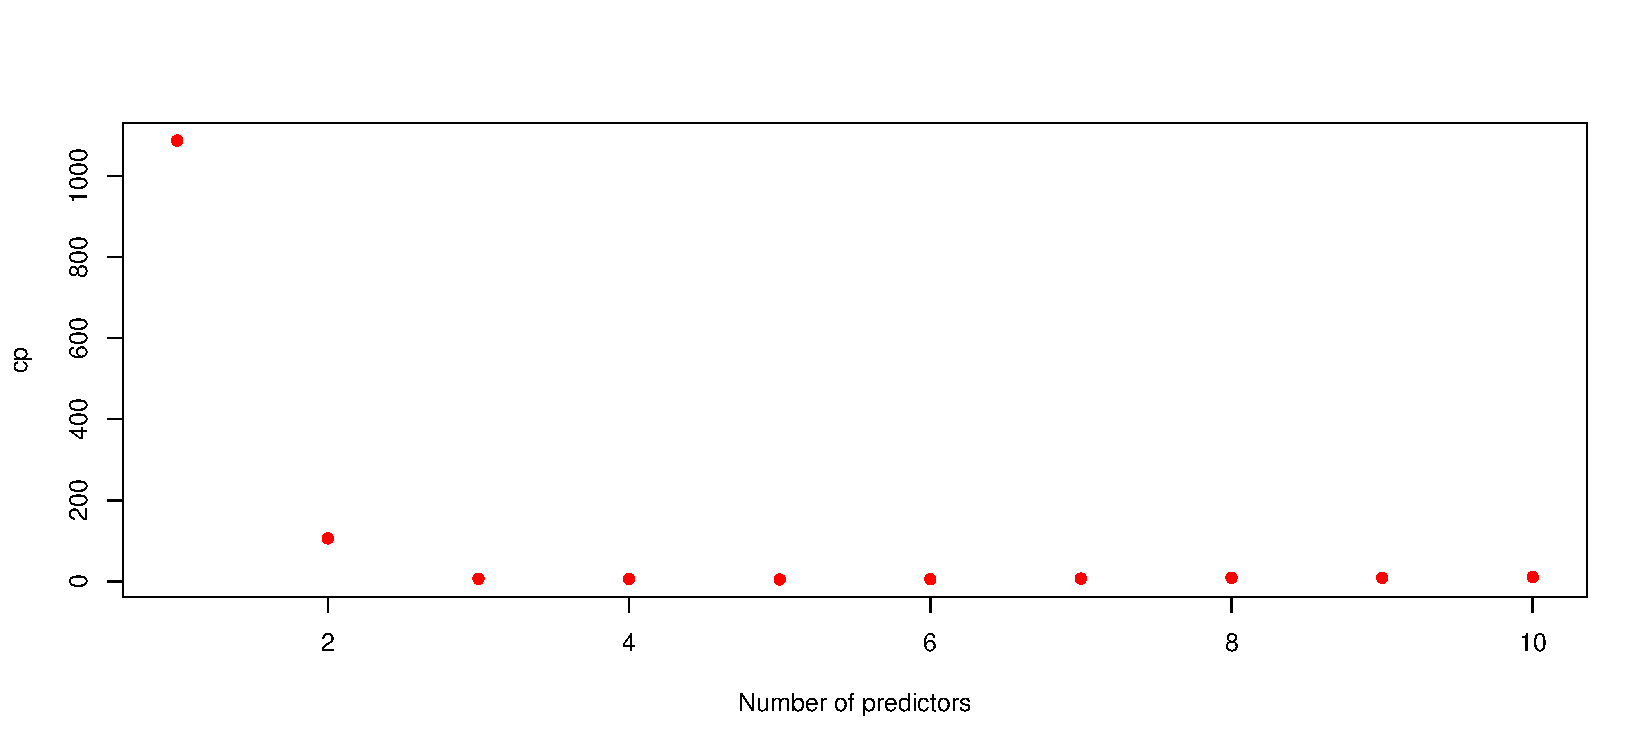
\includegraphics{hw2_fall18_files/figure-latex/unnamed-chunk-4-1.pdf}

\begin{Shaded}
\begin{Highlighting}[]
\KeywordTok{plot}\NormalTok{(new_summary}\OperatorTok{$}\NormalTok{bic, }\DataTypeTok{xlab=}\StringTok{"Number of predictors"}\NormalTok{, }
     \DataTypeTok{ylab=}\StringTok{"bic"}\NormalTok{, }\DataTypeTok{col=}\StringTok{"blue"}\NormalTok{, }\DataTypeTok{type=}\StringTok{"p"}\NormalTok{, }\DataTypeTok{pch=}\DecValTok{16}\NormalTok{)}
\end{Highlighting}
\end{Shaded}

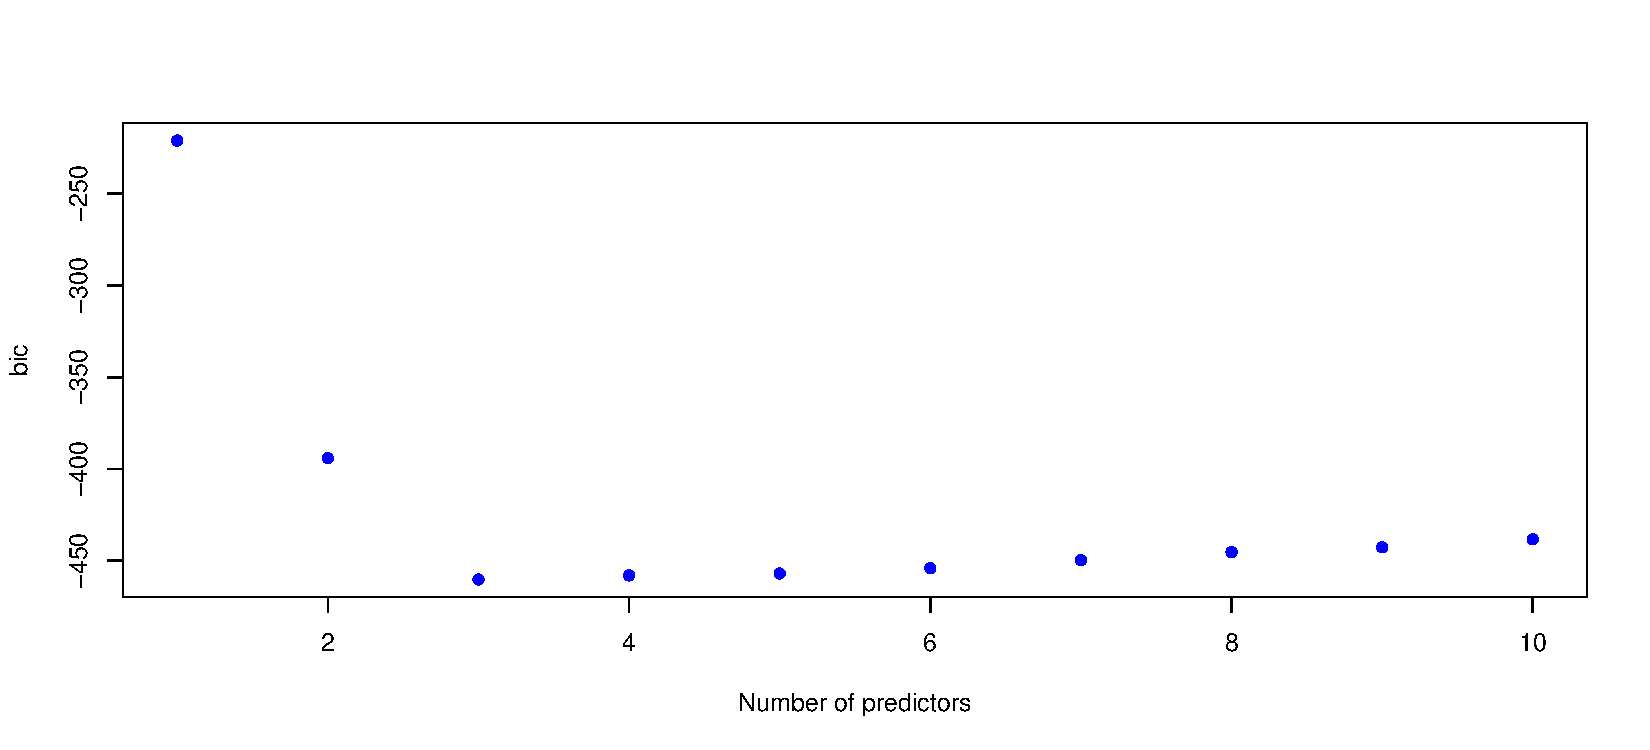
\includegraphics{hw2_fall18_files/figure-latex/unnamed-chunk-4-2.pdf}

\begin{Shaded}
\begin{Highlighting}[]
\KeywordTok{plot}\NormalTok{(new_summary}\OperatorTok{$}\NormalTok{adjr2, }\DataTypeTok{xlab=}\StringTok{"Number of predictors"}\NormalTok{, }
     \DataTypeTok{ylab=}\StringTok{"adjr2"}\NormalTok{, }\DataTypeTok{col=}\StringTok{"green"}\NormalTok{, }\DataTypeTok{type=}\StringTok{"p"}\NormalTok{, }\DataTypeTok{pch=}\DecValTok{16}\NormalTok{)}
\end{Highlighting}
\end{Shaded}

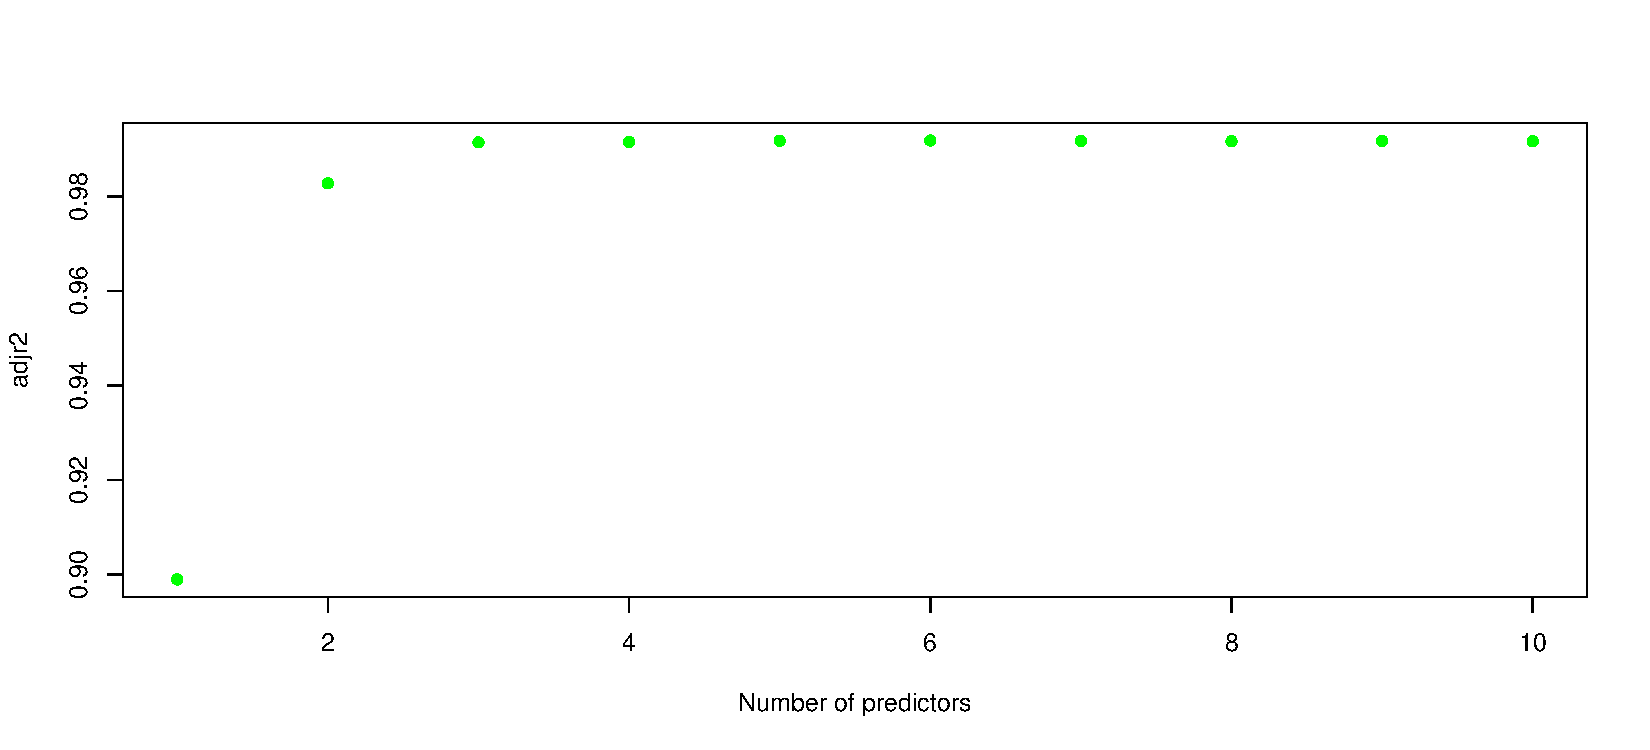
\includegraphics{hw2_fall18_files/figure-latex/unnamed-chunk-4-3.pdf}

\begin{Shaded}
\begin{Highlighting}[]
\CommentTok{# Find the optimal model size for Cp}
\NormalTok{opt.size <-}\StringTok{ }\KeywordTok{which.min}\NormalTok{(new_summary}\OperatorTok{$}\NormalTok{cp)}
\NormalTok{opt.size}
\end{Highlighting}
\end{Shaded}

\begin{verbatim}
## [1] 6
\end{verbatim}

\begin{Shaded}
\begin{Highlighting}[]
\CommentTok{# Find the optimal model size for bic}
\NormalTok{opt.size <-}\StringTok{ }\KeywordTok{which.min}\NormalTok{(new_summary}\OperatorTok{$}\NormalTok{bic)}
\NormalTok{opt.size}
\end{Highlighting}
\end{Shaded}

\begin{verbatim}
## [1] 3
\end{verbatim}

\begin{Shaded}
\begin{Highlighting}[]
\CommentTok{# Find the optimal model size for r2}
\NormalTok{opt.size <-}\StringTok{ }\KeywordTok{which.min}\NormalTok{(new_summary}\OperatorTok{$}\NormalTok{rsq)}
\NormalTok{opt.size}
\end{Highlighting}
\end{Shaded}

\begin{verbatim}
## [1] 1
\end{verbatim}

\begin{Shaded}
\begin{Highlighting}[]
\CommentTok{# Report the coefficients of the best model obtained}
\KeywordTok{coef}\NormalTok{(new_subset, }\DecValTok{3}\NormalTok{)}
\end{Highlighting}
\end{Shaded}

\begin{verbatim}
## (Intercept)           x          x2          x3 
##   0.8941296   1.9814762   3.1007060   4.0124572
\end{verbatim}

\begin{enumerate}
\def\labelenumi{(\alph{enumi})}
\setcounter{enumi}{3}
\item
\end{enumerate}

\begin{Shaded}
\begin{Highlighting}[]
\CommentTok{# Repeat using forward selection}
\NormalTok{forward <-}\StringTok{ }\KeywordTok{regsubsets}\NormalTok{(y }\OperatorTok{~}\StringTok{ }\NormalTok{x}\OperatorTok{+}\NormalTok{x2}\OperatorTok{+}\NormalTok{x3}\OperatorTok{+}\NormalTok{x4}\OperatorTok{+}\NormalTok{x5}\OperatorTok{+}\NormalTok{x6}\OperatorTok{+}\NormalTok{x7}\OperatorTok{+}\NormalTok{x8}\OperatorTok{+}\NormalTok{x9}\OperatorTok{+}\NormalTok{x10,}\DataTypeTok{data =}\NormalTok{ new_data, }\DataTypeTok{nvmax =} \DecValTok{10}\NormalTok{, }\DataTypeTok{method =} \StringTok{"forward"}\NormalTok{)}
\NormalTok{forward_sum <-}\StringTok{ }\KeywordTok{summary}\NormalTok{(forward)}
\NormalTok{forward_sum}
\end{Highlighting}
\end{Shaded}

\begin{verbatim}
## Subset selection object
## Call: regsubsets.formula(y ~ x + x2 + x3 + x4 + x5 + x6 + x7 + x8 + 
##     x9 + x10, data = new_data, nvmax = 10, method = "forward")
## 10 Variables  (and intercept)
##     Forced in Forced out
## x       FALSE      FALSE
## x2      FALSE      FALSE
## x3      FALSE      FALSE
## x4      FALSE      FALSE
## x5      FALSE      FALSE
## x6      FALSE      FALSE
## x7      FALSE      FALSE
## x8      FALSE      FALSE
## x9      FALSE      FALSE
## x10     FALSE      FALSE
## 1 subsets of each size up to 10
## Selection Algorithm: forward
##           x   x2  x3  x4  x5  x6  x7  x8  x9  x10
## 1  ( 1 )  " " " " "*" " " " " " " " " " " " " " "
## 2  ( 1 )  " " "*" "*" " " " " " " " " " " " " " "
## 3  ( 1 )  "*" "*" "*" " " " " " " " " " " " " " "
## 4  ( 1 )  "*" "*" "*" " " " " " " " " " " "*" " "
## 5  ( 1 )  "*" "*" "*" " " " " " " "*" " " "*" " "
## 6  ( 1 )  "*" "*" "*" "*" " " " " "*" " " "*" " "
## 7  ( 1 )  "*" "*" "*" "*" "*" " " "*" " " "*" " "
## 8  ( 1 )  "*" "*" "*" "*" "*" " " "*" " " "*" "*"
## 9  ( 1 )  "*" "*" "*" "*" "*" "*" "*" " " "*" "*"
## 10  ( 1 ) "*" "*" "*" "*" "*" "*" "*" "*" "*" "*"
\end{verbatim}

\begin{Shaded}
\begin{Highlighting}[]
\KeywordTok{plot}\NormalTok{(forward_sum}\OperatorTok{$}\NormalTok{rsq, }\DataTypeTok{ylab=}\StringTok{"rsq"}\NormalTok{, }\DataTypeTok{col=}\StringTok{"red"}\NormalTok{, }\DataTypeTok{type=}\StringTok{"p"}\NormalTok{, }\DataTypeTok{pch=}\DecValTok{16}\NormalTok{,}
     \DataTypeTok{xlab=}\StringTok{"Forward Selection"}\NormalTok{)}
\end{Highlighting}
\end{Shaded}

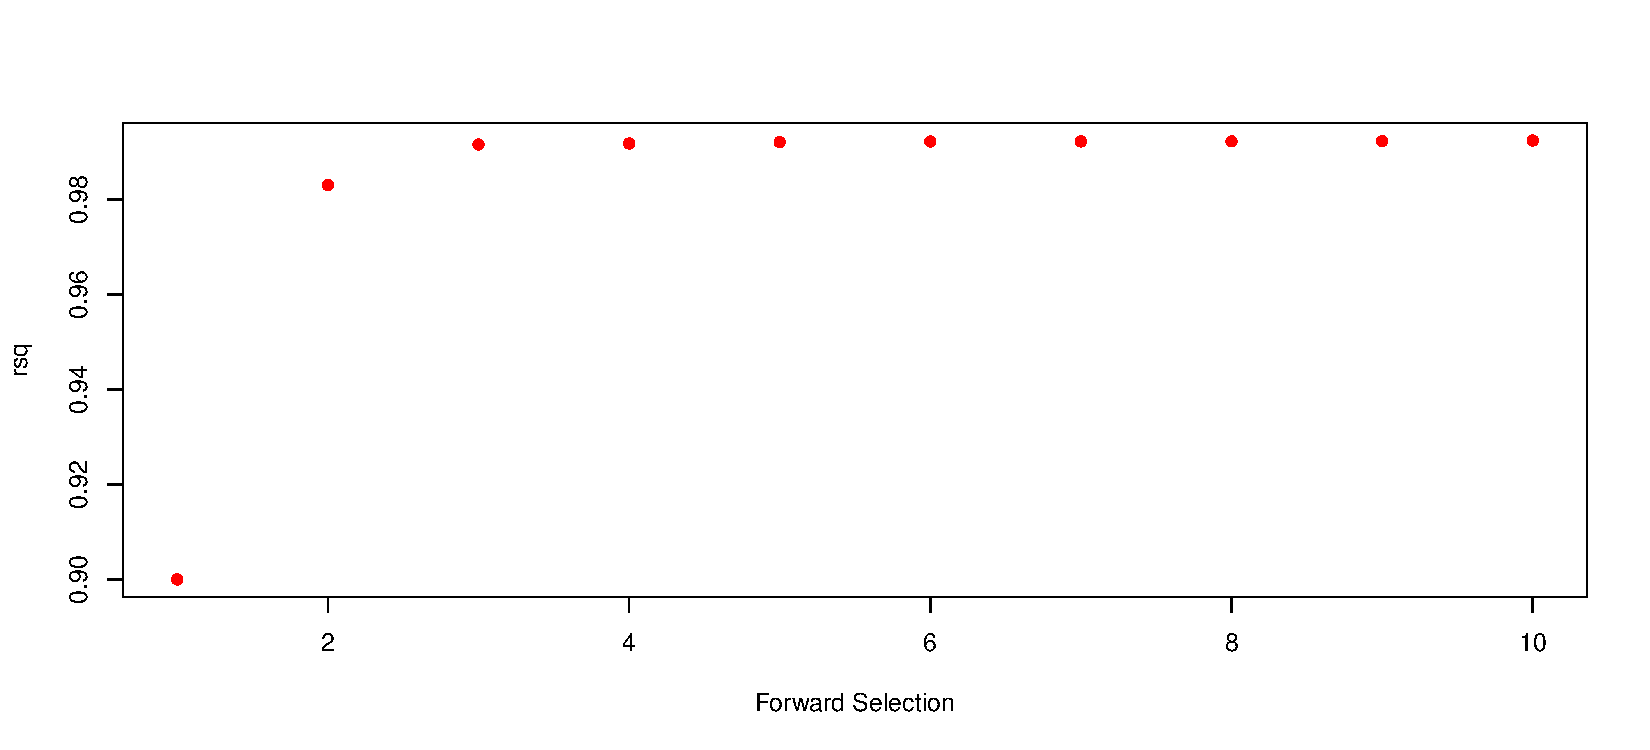
\includegraphics{hw2_fall18_files/figure-latex/unnamed-chunk-5-1.pdf}

\begin{Shaded}
\begin{Highlighting}[]
\CommentTok{# Find the optimal model size for forward selection}
\NormalTok{opt.size <-}\StringTok{ }\KeywordTok{which.min}\NormalTok{(forward_sum}\OperatorTok{$}\NormalTok{rsq)}
\NormalTok{opt.size}
\end{Highlighting}
\end{Shaded}

\begin{verbatim}
## [1] 1
\end{verbatim}

\begin{Shaded}
\begin{Highlighting}[]
\CommentTok{# Report the coefficients for forward selection}
\KeywordTok{coef}\NormalTok{(forward, }\DecValTok{3}\NormalTok{)}
\end{Highlighting}
\end{Shaded}

\begin{verbatim}
## (Intercept)           x          x2          x3 
##   0.8941296   1.9814762   3.1007060   4.0124572
\end{verbatim}

\begin{Shaded}
\begin{Highlighting}[]
\CommentTok{# Repeat using backward selection}
\NormalTok{backward <-}\StringTok{ }\KeywordTok{regsubsets}\NormalTok{(y }\OperatorTok{~}\StringTok{ }\NormalTok{x}\OperatorTok{+}\NormalTok{x2}\OperatorTok{+}\NormalTok{x3}\OperatorTok{+}\NormalTok{x4}\OperatorTok{+}\NormalTok{x5}\OperatorTok{+}\NormalTok{x6}\OperatorTok{+}\NormalTok{x7}\OperatorTok{+}\NormalTok{x8}\OperatorTok{+}\NormalTok{x9}\OperatorTok{+}\NormalTok{x10,}\DataTypeTok{data =}\NormalTok{ new_data, }\DataTypeTok{nvmax =} \DecValTok{10}\NormalTok{, }\DataTypeTok{method =} \StringTok{"backward"}\NormalTok{)}
\NormalTok{backward_sum <-}\StringTok{ }\KeywordTok{summary}\NormalTok{(backward)}
\NormalTok{backward_sum}
\end{Highlighting}
\end{Shaded}

\begin{verbatim}
## Subset selection object
## Call: regsubsets.formula(y ~ x + x2 + x3 + x4 + x5 + x6 + x7 + x8 + 
##     x9 + x10, data = new_data, nvmax = 10, method = "backward")
## 10 Variables  (and intercept)
##     Forced in Forced out
## x       FALSE      FALSE
## x2      FALSE      FALSE
## x3      FALSE      FALSE
## x4      FALSE      FALSE
## x5      FALSE      FALSE
## x6      FALSE      FALSE
## x7      FALSE      FALSE
## x8      FALSE      FALSE
## x9      FALSE      FALSE
## x10     FALSE      FALSE
## 1 subsets of each size up to 10
## Selection Algorithm: backward
##           x   x2  x3  x4  x5  x6  x7  x8  x9  x10
## 1  ( 1 )  " " " " "*" " " " " " " " " " " " " " "
## 2  ( 1 )  " " "*" "*" " " " " " " " " " " " " " "
## 3  ( 1 )  "*" "*" "*" " " " " " " " " " " " " " "
## 4  ( 1 )  "*" "*" "*" " " " " " " " " "*" " " " "
## 5  ( 1 )  "*" "*" "*" " " " " "*" " " "*" " " " "
## 6  ( 1 )  "*" "*" "*" " " " " "*" "*" "*" " " " "
## 7  ( 1 )  "*" "*" "*" "*" " " "*" "*" "*" " " " "
## 8  ( 1 )  "*" "*" "*" "*" "*" "*" "*" "*" " " " "
## 9  ( 1 )  "*" "*" "*" "*" "*" "*" "*" "*" " " "*"
## 10  ( 1 ) "*" "*" "*" "*" "*" "*" "*" "*" "*" "*"
\end{verbatim}

\begin{Shaded}
\begin{Highlighting}[]
\KeywordTok{plot}\NormalTok{(backward_sum}\OperatorTok{$}\NormalTok{rsq, }\DataTypeTok{ylab=}\StringTok{"rsq"}\NormalTok{, }\DataTypeTok{col=}\StringTok{"red"}\NormalTok{, }\DataTypeTok{type=}\StringTok{"p"}\NormalTok{, }\DataTypeTok{pch=}\DecValTok{16}\NormalTok{,}
     \DataTypeTok{xlab=}\StringTok{"Backward Selection"}\NormalTok{)}
\end{Highlighting}
\end{Shaded}

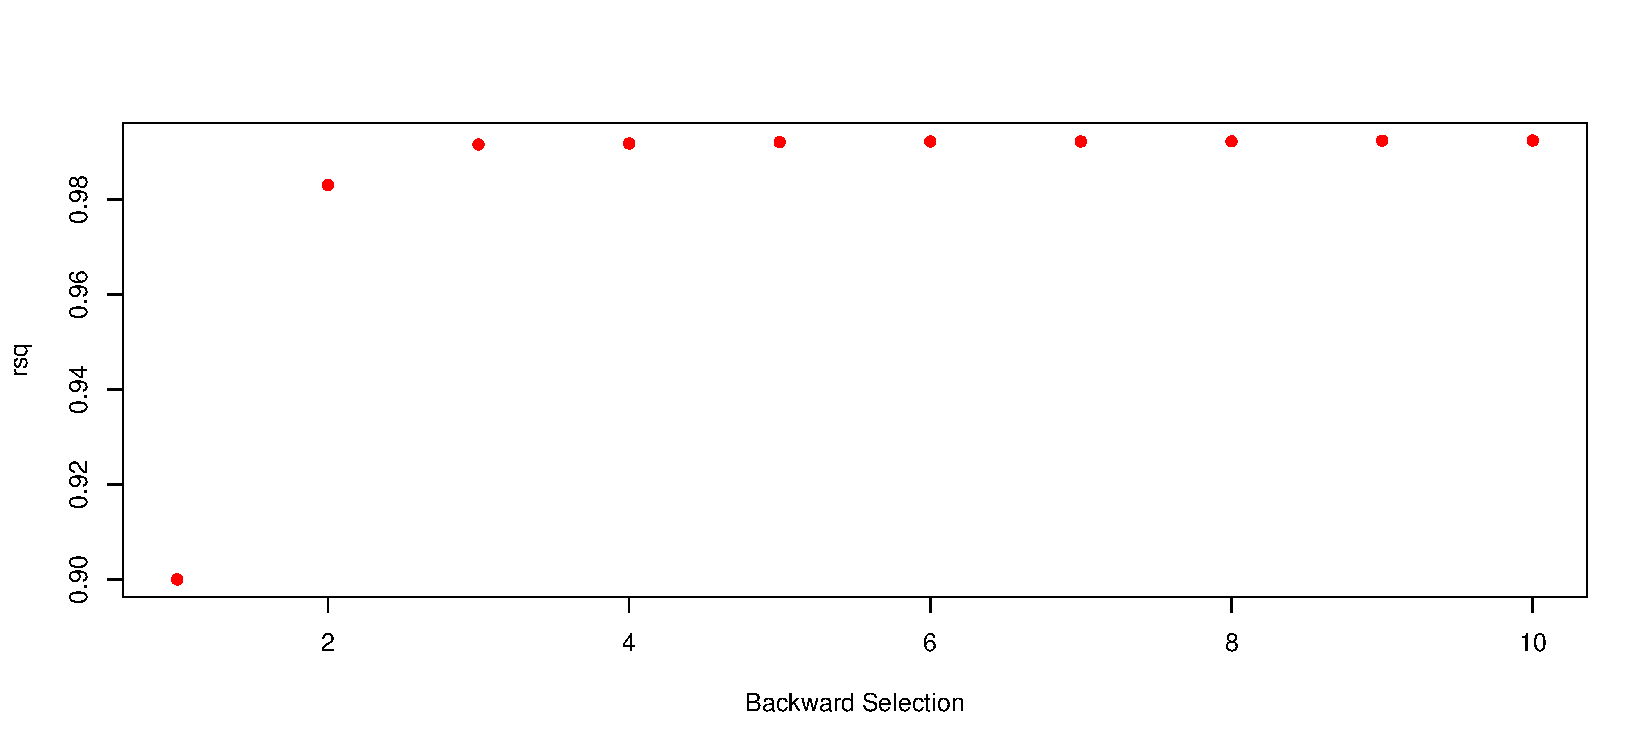
\includegraphics{hw2_fall18_files/figure-latex/unnamed-chunk-5-2.pdf}

\begin{Shaded}
\begin{Highlighting}[]
\CommentTok{# Find the optimal model size for backward selection}
\NormalTok{opt.size <-}\StringTok{ }\KeywordTok{which.min}\NormalTok{(backward_sum}\OperatorTok{$}\NormalTok{rsq)}
\NormalTok{opt.size}
\end{Highlighting}
\end{Shaded}

\begin{verbatim}
## [1] 1
\end{verbatim}

\begin{Shaded}
\begin{Highlighting}[]
\CommentTok{# Report the coefficients for backward selection}
\KeywordTok{coef}\NormalTok{(backward, }\DecValTok{3}\NormalTok{)}
\end{Highlighting}
\end{Shaded}

\begin{verbatim}
## (Intercept)           x          x2          x3 
##   0.8941296   1.9814762   3.1007060   4.0124572
\end{verbatim}

Using forward and backward stepwise selection, we only use one variable
(x3) as opposed to three variables (x, x2, x3).

\begin{enumerate}
\def\labelenumi{(\alph{enumi})}
\setcounter{enumi}{4}
\item
\end{enumerate}

Describe what Cp and BIC are estimating.

Cp: an unbiased estimator of average prediction errors.

BIC: uses k to estimate the number of parameters. It heavily penalizes
additional variables when they are introduced into the model. Therefore,
BIC models tend to have fewer variables.

\subsection{Problem 2:}\label{problem-2}

This will be the last part of the Auto data from ISLR. The original data
contains 408 observations about cars. It has some similarity as the data
CARS that we use in our lectures. To get the data, first install the
package ISLR. The data Auto should be loaded automatically. We use this
case to go through methods learnt so far.

You can access the necessary data with the following code:

\begin{Shaded}
\begin{Highlighting}[]
\CommentTok{# check if you have ISLR package, if not, install it}
\ControlFlowTok{if}\NormalTok{(}\OperatorTok{!}\KeywordTok{requireNamespace}\NormalTok{(}\StringTok{'ISLR'}\NormalTok{)) }\KeywordTok{install.packages}\NormalTok{(}\StringTok{'ISLR'}\NormalTok{) }
\NormalTok{auto <-}\StringTok{ }\NormalTok{ISLR}\OperatorTok{::}\NormalTok{Auto}
\end{Highlighting}
\end{Shaded}

Final modelling question: we want to explore the effects of each feature
as best as possible. You may explore interactions, feature
transformations, higher order terms, or other strategies within reason.
The model(s) should be as parsimonious (simple) as possible unless the
gain in accuracy is significant from your point of view. Use Mallow's Cp
or BIC to select the model. * Describe the final model and its accuracy.
Include diagnostic plots with particular focus on the model residuals. *
Summarize the effects found. * Predict the mpg of a car that is: built
in 1983, in US, red, 180 inches long, 8 cylinders, 350 displacement, 260
as horsepower and weighs 4000 pounds. Give a 95\% CI.

\begin{Shaded}
\begin{Highlighting}[]
\KeywordTok{dim}\NormalTok{(auto)}
\end{Highlighting}
\end{Shaded}

\begin{verbatim}
## [1] 392   9
\end{verbatim}

\begin{Shaded}
\begin{Highlighting}[]
\KeywordTok{str}\NormalTok{(auto)}
\end{Highlighting}
\end{Shaded}

\begin{verbatim}
## 'data.frame':    392 obs. of  9 variables:
##  $ mpg         : num  18 15 18 16 17 15 14 14 14 15 ...
##  $ cylinders   : num  8 8 8 8 8 8 8 8 8 8 ...
##  $ displacement: num  307 350 318 304 302 429 454 440 455 390 ...
##  $ horsepower  : num  130 165 150 150 140 198 220 215 225 190 ...
##  $ weight      : num  3504 3693 3436 3433 3449 ...
##  $ acceleration: num  12 11.5 11 12 10.5 10 9 8.5 10 8.5 ...
##  $ year        : num  70 70 70 70 70 70 70 70 70 70 ...
##  $ origin      : num  1 1 1 1 1 1 1 1 1 1 ...
##  $ name        : Factor w/ 304 levels "amc ambassador brougham",..: 49 36 231 14 161 141 54 223 241 2 ...
\end{verbatim}

\begin{Shaded}
\begin{Highlighting}[]
\CommentTok{#Exclude non-numeric values, and run pairwise scatter plot}
\NormalTok{auto }\OperatorTok
\StringTok{  }\KeywordTok{select_if}\NormalTok{(is.numeric) }\OperatorTok
\StringTok{  }\KeywordTok{pairs}\NormalTok{()}
\end{Highlighting}
\end{Shaded}

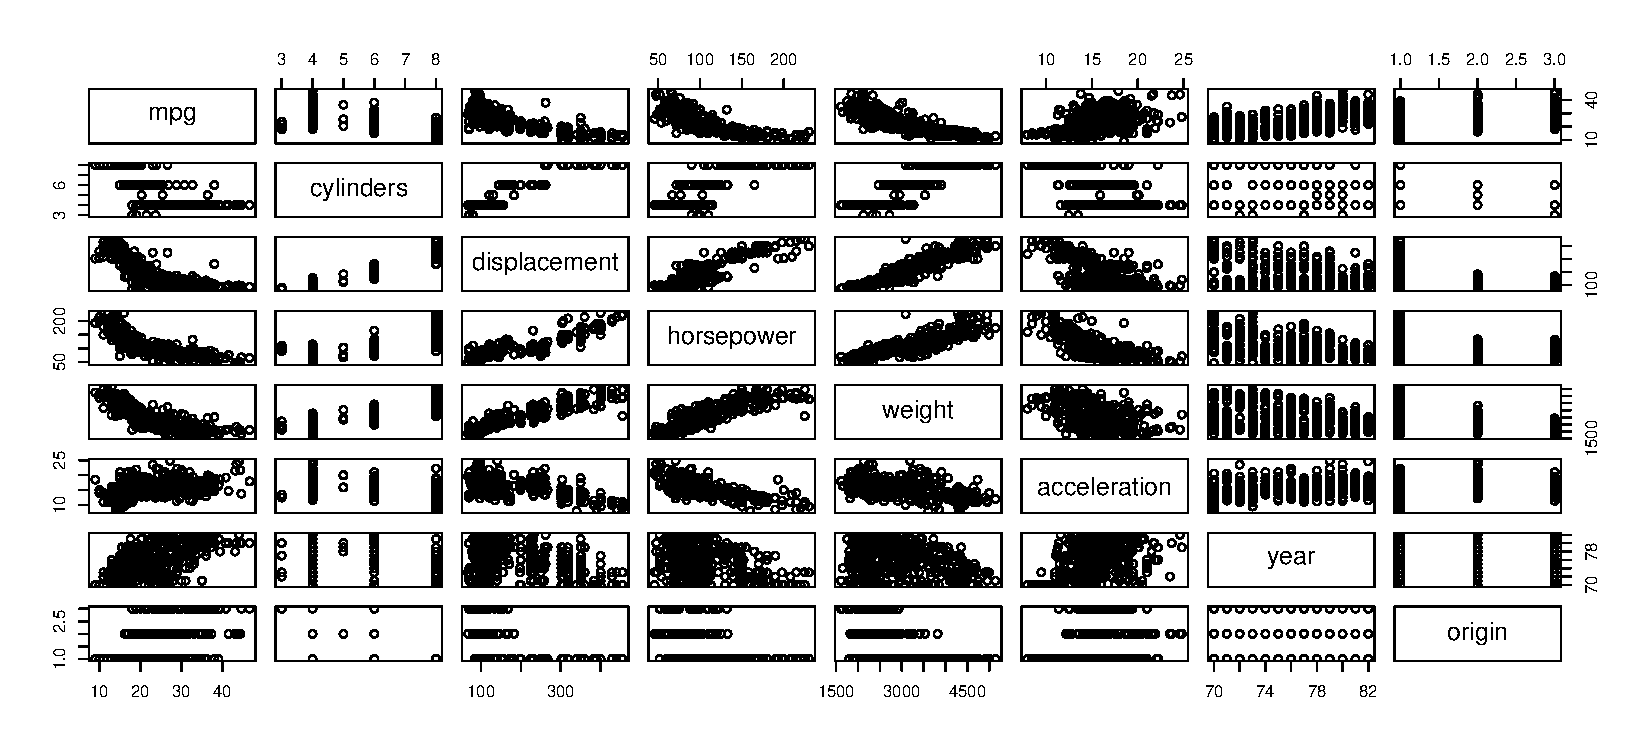
\includegraphics{hw2_fall18_files/figure-latex/unnamed-chunk-7-1.pdf}

\begin{Shaded}
\begin{Highlighting}[]
\CommentTok{#From this we can see that MPG is highly correlated with Displacement, Horsepower and Weight}
\end{Highlighting}
\end{Shaded}

\begin{Shaded}
\begin{Highlighting}[]
\CommentTok{#Use Regsubsets to find the model with the smallest RSS }
\KeywordTok{names}\NormalTok{(auto)}
\end{Highlighting}
\end{Shaded}

\begin{verbatim}
## [1] "mpg"          "cylinders"    "displacement" "horsepower"  
## [5] "weight"       "acceleration" "year"         "origin"      
## [9] "name"
\end{verbatim}

\begin{Shaded}
\begin{Highlighting}[]
\NormalTok{data2 <-}\StringTok{ }\NormalTok{auto[,}\OperatorTok{-}\DecValTok{9}\NormalTok{]}
\NormalTok{fit.exh <-}\StringTok{ }\KeywordTok{regsubsets}\NormalTok{(mpg}\OperatorTok{~}\StringTok{ }\NormalTok{.,data2,}\DataTypeTok{nvmax =} \DecValTok{25}\NormalTok{, }\DataTypeTok{method =} \StringTok{"exhaustive"}\NormalTok{)}
\KeywordTok{names}\NormalTok{(fit.exh)}
\end{Highlighting}
\end{Shaded}

\begin{verbatim}
##  [1] "np"        "nrbar"     "d"         "rbar"      "thetab"   
##  [6] "first"     "last"      "vorder"    "tol"       "rss"      
## [11] "bound"     "nvmax"     "ress"      "ir"        "nbest"    
## [16] "lopt"      "il"        "ier"       "xnames"    "method"   
## [21] "force.in"  "force.out" "sserr"     "intercept" "lindep"   
## [26] "nullrss"   "nn"        "call"
\end{verbatim}

\begin{Shaded}
\begin{Highlighting}[]
\CommentTok{#List the model with the smallest RSS among each size of the model}
\KeywordTok{summary}\NormalTok{(fit.exh)}
\end{Highlighting}
\end{Shaded}

\begin{verbatim}
## Subset selection object
## Call: regsubsets.formula(mpg ~ ., data2, nvmax = 25, method = "exhaustive")
## 7 Variables  (and intercept)
##              Forced in Forced out
## cylinders        FALSE      FALSE
## displacement     FALSE      FALSE
## horsepower       FALSE      FALSE
## weight           FALSE      FALSE
## acceleration     FALSE      FALSE
## year             FALSE      FALSE
## origin           FALSE      FALSE
## 1 subsets of each size up to 7
## Selection Algorithm: exhaustive
##          cylinders displacement horsepower weight acceleration year origin
## 1  ( 1 ) " "       " "          " "        "*"    " "          " "  " "   
## 2  ( 1 ) " "       " "          " "        "*"    " "          "*"  " "   
## 3  ( 1 ) " "       " "          " "        "*"    " "          "*"  "*"   
## 4  ( 1 ) " "       "*"          " "        "*"    " "          "*"  "*"   
## 5  ( 1 ) " "       "*"          "*"        "*"    " "          "*"  "*"   
## 6  ( 1 ) "*"       "*"          "*"        "*"    " "          "*"  "*"   
## 7  ( 1 ) "*"       "*"          "*"        "*"    "*"          "*"  "*"
\end{verbatim}

\begin{Shaded}
\begin{Highlighting}[]
\NormalTok{f.e<-}\KeywordTok{summary}\NormalTok{(fit.exh)}
\NormalTok{f.e}\OperatorTok{$}\NormalTok{which}
\end{Highlighting}
\end{Shaded}

\begin{verbatim}
##   (Intercept) cylinders displacement horsepower weight acceleration  year
## 1        TRUE     FALSE        FALSE      FALSE   TRUE        FALSE FALSE
## 2        TRUE     FALSE        FALSE      FALSE   TRUE        FALSE  TRUE
## 3        TRUE     FALSE        FALSE      FALSE   TRUE        FALSE  TRUE
## 4        TRUE     FALSE         TRUE      FALSE   TRUE        FALSE  TRUE
## 5        TRUE     FALSE         TRUE       TRUE   TRUE        FALSE  TRUE
## 6        TRUE      TRUE         TRUE       TRUE   TRUE        FALSE  TRUE
## 7        TRUE      TRUE         TRUE       TRUE   TRUE         TRUE  TRUE
##   origin
## 1  FALSE
## 2  FALSE
## 3   TRUE
## 4   TRUE
## 5   TRUE
## 6   TRUE
## 7   TRUE
\end{verbatim}

\begin{Shaded}
\begin{Highlighting}[]
\KeywordTok{data.frame}\NormalTok{(}\DataTypeTok{variables=}\NormalTok{(}\DecValTok{1}\OperatorTok{:}\KeywordTok{length}\NormalTok{(f.e}\OperatorTok{$}\NormalTok{rsq)), }\DataTypeTok{r_squared=}\NormalTok{f.e}\OperatorTok{$}\NormalTok{rsq)}
\end{Highlighting}
\end{Shaded}

\begin{verbatim}
##   variables r_squared
## 1         1 0.6926304
## 2         2 0.8081803
## 3         3 0.8174522
## 4         4 0.8180977
## 5         5 0.8200242
## 6         6 0.8211691
## 7         7 0.8214781
\end{verbatim}

\begin{Shaded}
\begin{Highlighting}[]
\CommentTok{#R2 increases as we increase number of variables (But much less incrementally so, after adding 2 variables)}
\end{Highlighting}
\end{Shaded}

\begin{Shaded}
\begin{Highlighting}[]
\KeywordTok{data.frame}\NormalTok{(}\DataTypeTok{variables =}\NormalTok{ (}\DecValTok{1}\OperatorTok{:}\KeywordTok{length}\NormalTok{(f.e}\OperatorTok{$}\NormalTok{rsq)),}
           \DataTypeTok{r_squared =}\NormalTok{ f.e}\OperatorTok{$}\NormalTok{rsq,}
           \DataTypeTok{rss =}\NormalTok{ f.e}\OperatorTok{$}\NormalTok{rss,}
           \DataTypeTok{bic =}\NormalTok{ f.e}\OperatorTok{$}\NormalTok{bic,}
           \DataTypeTok{cp =}\NormalTok{ f.e}\OperatorTok{$}\NormalTok{cp)}
\end{Highlighting}
\end{Shaded}

\begin{verbatim}
##   variables r_squared      rss       bic         cp
## 1         1 0.6926304 7321.234 -450.5016 273.150806
## 2         2 0.8081803 4568.952 -629.3564  26.603456
## 3         3 0.8174522 4348.105 -642.8063   8.659680
## 4         4 0.8180977 4332.729 -638.2237   9.271088
## 5         5 0.8200242 4286.842 -636.4261   7.127265
## 6         6 0.8211691 4259.571 -632.9566   6.664509
## 7         7 0.8214781 4252.213 -627.6631   8.000000
\end{verbatim}

\begin{Shaded}
\begin{Highlighting}[]
\KeywordTok{coef}\NormalTok{(fit.exh, }\DecValTok{6}\NormalTok{)}
\end{Highlighting}
\end{Shaded}

\begin{verbatim}
##   (Intercept)     cylinders  displacement    horsepower        weight 
## -15.563492306  -0.506685137   0.019269286  -0.023895029  -0.006218311 
##          year        origin 
##   0.747515952   1.428241885
\end{verbatim}

\begin{Shaded}
\begin{Highlighting}[]
\KeywordTok{coef}\NormalTok{(fit.exh, }\DecValTok{7}\NormalTok{)}
\end{Highlighting}
\end{Shaded}

\begin{verbatim}
##   (Intercept)     cylinders  displacement    horsepower        weight 
## -17.218434622  -0.493376319   0.019895644  -0.016951144  -0.006474043 
##  acceleration          year        origin 
##   0.080575838   0.750772678   1.426140495
\end{verbatim}

plots of \(Cp\) vs number of predictors and plots of \(BIC\) vs number
of the predictors

\begin{Shaded}
\begin{Highlighting}[]
\KeywordTok{plot}\NormalTok{(f.e}\OperatorTok{$}\NormalTok{cp, }\DataTypeTok{xlab=}\StringTok{"Number of predictors"}\NormalTok{, }
     \DataTypeTok{ylab=}\StringTok{"cp"}\NormalTok{, }\DataTypeTok{col=}\StringTok{"red"}\NormalTok{, }\DataTypeTok{type=}\StringTok{"p"}\NormalTok{, }\DataTypeTok{pch=}\DecValTok{16}\NormalTok{)}
\end{Highlighting}
\end{Shaded}

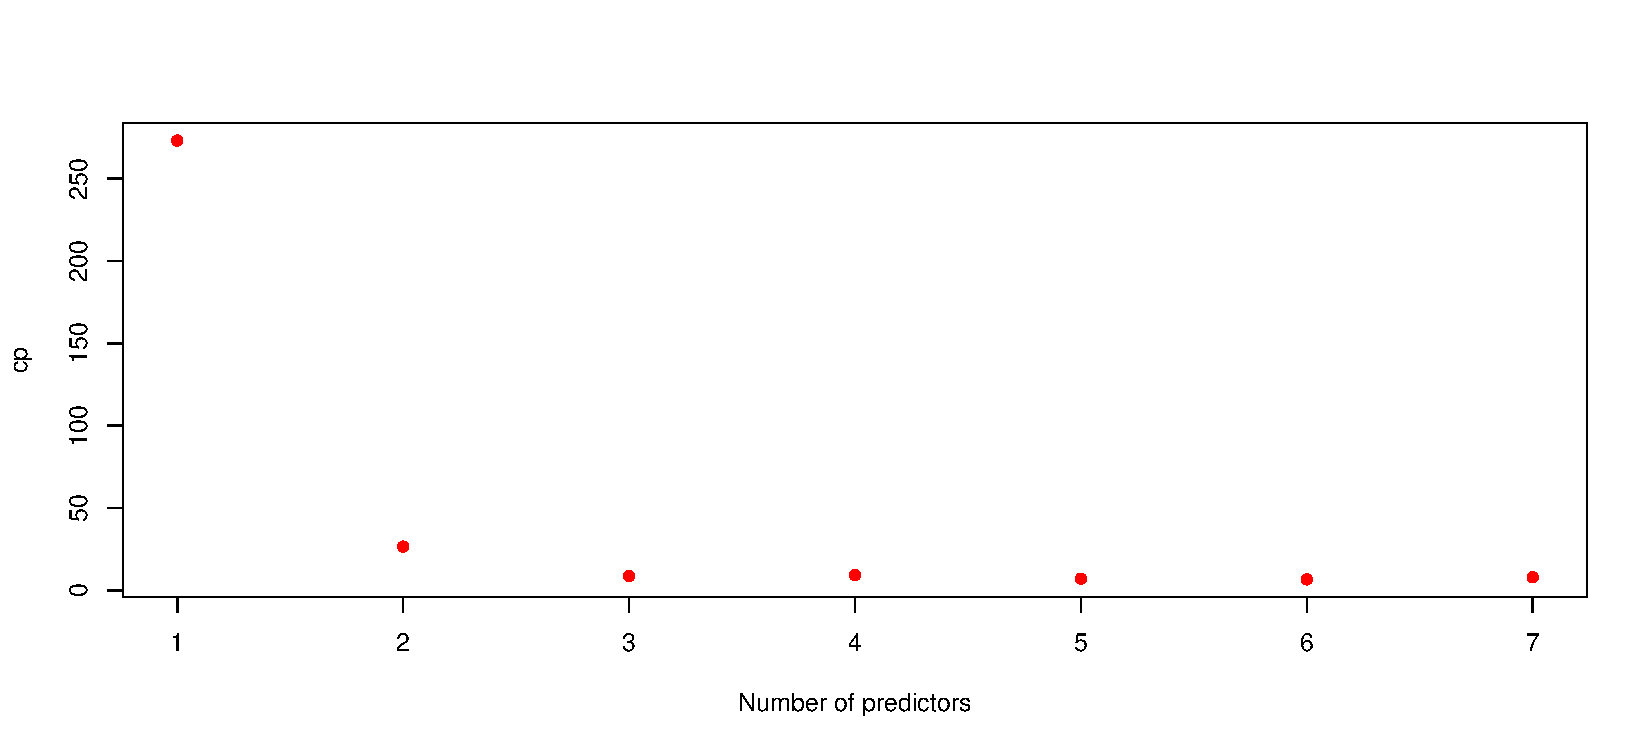
\includegraphics{hw2_fall18_files/figure-latex/unnamed-chunk-13-1.pdf}

\begin{Shaded}
\begin{Highlighting}[]
\CommentTok{#CP smallest at 6 variables}
\KeywordTok{plot}\NormalTok{(f.e}\OperatorTok{$}\NormalTok{bic, }\DataTypeTok{xlab=}\StringTok{"Number of predictors"}\NormalTok{, }
     \DataTypeTok{ylab=}\StringTok{"bic"}\NormalTok{, }\DataTypeTok{col=}\StringTok{"blue"}\NormalTok{, }\DataTypeTok{type=}\StringTok{"p"}\NormalTok{, }\DataTypeTok{pch=}\DecValTok{16}\NormalTok{)}
\end{Highlighting}
\end{Shaded}

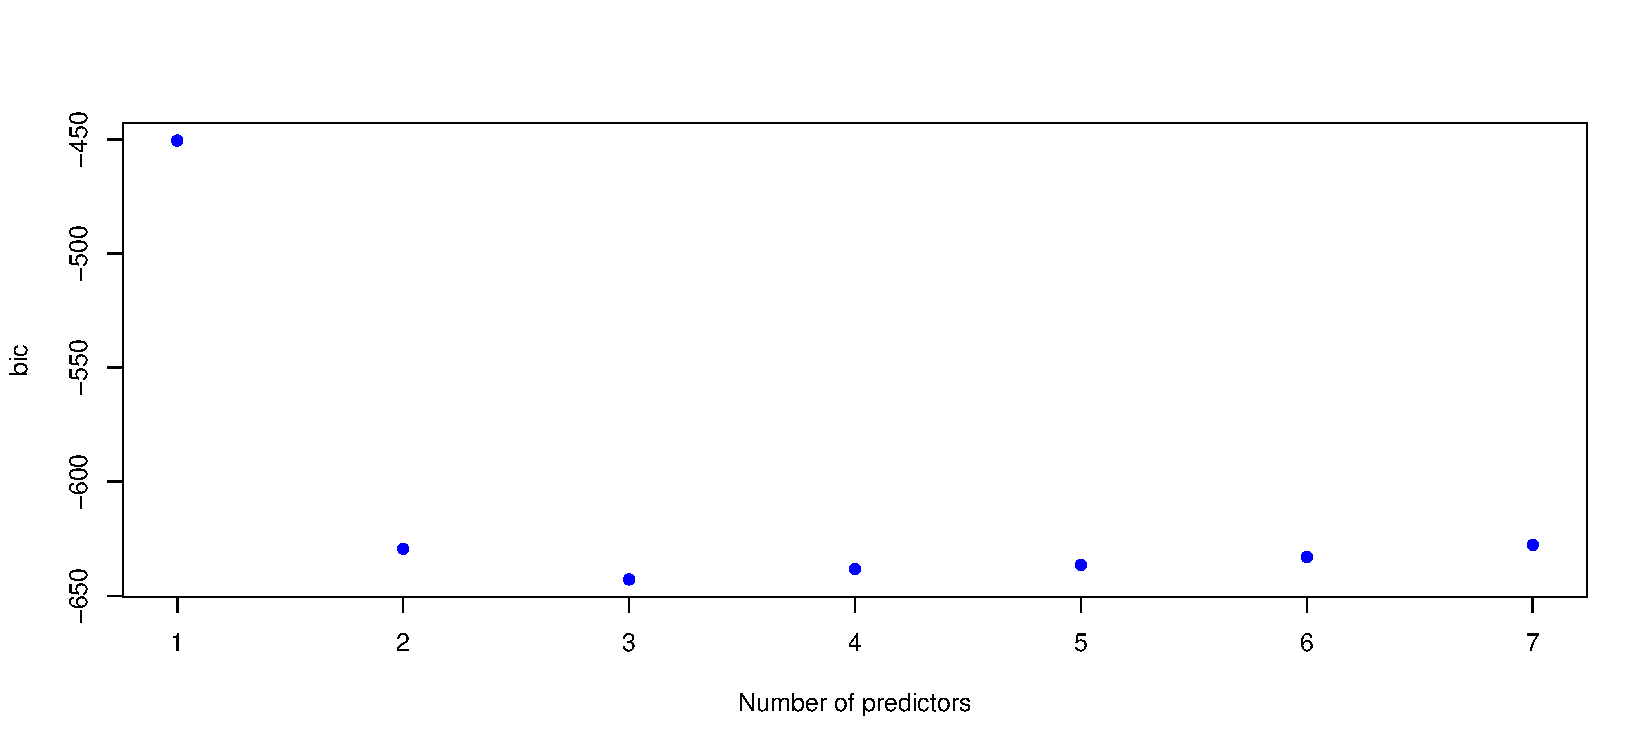
\includegraphics{hw2_fall18_files/figure-latex/unnamed-chunk-13-2.pdf}

\begin{Shaded}
\begin{Highlighting}[]
\CommentTok{#BIC smallest at 3 variables}
\end{Highlighting}
\end{Shaded}

\begin{Shaded}
\begin{Highlighting}[]
\KeywordTok{which.min}\NormalTok{(f.e}\OperatorTok{$}\NormalTok{cp)}
\end{Highlighting}
\end{Shaded}

\begin{verbatim}
## [1] 6
\end{verbatim}

\begin{Shaded}
\begin{Highlighting}[]
\KeywordTok{which.min}\NormalTok{(f.e}\OperatorTok{$}\NormalTok{bic) }\CommentTok{#Choose BIC}
\end{Highlighting}
\end{Shaded}

\begin{verbatim}
## [1] 3
\end{verbatim}

We may use 3 variable model (BIC tends to give the model with least
number of predictors)

\begin{Shaded}
\begin{Highlighting}[]
\NormalTok{fit.exh.var <-}\StringTok{ }\NormalTok{f.e}\OperatorTok{$}\NormalTok{which[}\DecValTok{3}\NormalTok{,]}
\KeywordTok{colnames}\NormalTok{(f.e}\OperatorTok{$}\NormalTok{which)[fit.exh.var] }
\end{Highlighting}
\end{Shaded}

\begin{verbatim}
## [1] "(Intercept)" "weight"      "year"        "origin"
\end{verbatim}

\section{\texorpdfstring{{[}1{]} ``(Intercept)'' ``weight'' ``year''
``origin''}{{[}1{]} (Intercept) weight year origin}}\label{intercept-weight-year-origin}

So we now have the three variables

\begin{Shaded}
\begin{Highlighting}[]
\NormalTok{fit.final <-}\StringTok{ }\KeywordTok{lm}\NormalTok{(mpg }\OperatorTok{~}\StringTok{ }\NormalTok{weight }\OperatorTok{+}\StringTok{ }\NormalTok{year }\OperatorTok{+}\StringTok{ }\NormalTok{origin, data2) }
\KeywordTok{summary}\NormalTok{(fit.final)}
\end{Highlighting}
\end{Shaded}

\begin{verbatim}
## 
## Call:
## lm(formula = mpg ~ weight + year + origin, data = data2)
## 
## Residuals:
##     Min      1Q  Median      3Q     Max 
## -9.9440 -2.0948 -0.0389  1.7255 13.2722 
## 
## Coefficients:
##               Estimate Std. Error t value Pr(>|t|)    
## (Intercept) -1.805e+01  4.001e+00  -4.510 8.60e-06 ***
## weight      -5.994e-03  2.541e-04 -23.588  < 2e-16 ***
## year         7.571e-01  4.832e-02  15.668  < 2e-16 ***
## origin       1.150e+00  2.591e-01   4.439 1.18e-05 ***
## ---
## Signif. codes:  0 '***' 0.001 '**' 0.01 '*' 0.05 '.' 0.1 ' ' 1
## 
## Residual standard error: 3.348 on 388 degrees of freedom
## Multiple R-squared:  0.8175, Adjusted R-squared:  0.816 
## F-statistic: 579.2 on 3 and 388 DF,  p-value: < 2.2e-16
\end{verbatim}

Final model with three variables

\begin{Shaded}
\begin{Highlighting}[]
\KeywordTok{par}\NormalTok{(}\DataTypeTok{mfrow=}\KeywordTok{c}\NormalTok{(}\DecValTok{1}\NormalTok{,}\DecValTok{2}\NormalTok{), }\DataTypeTok{mar=}\KeywordTok{c}\NormalTok{(}\FloatTok{2.5}\NormalTok{,}\DecValTok{3}\NormalTok{,}\FloatTok{1.5}\NormalTok{,}\DecValTok{1}\NormalTok{), }\DataTypeTok{mgp=}\KeywordTok{c}\NormalTok{(}\FloatTok{1.5}\NormalTok{,}\FloatTok{0.5}\NormalTok{,}\DecValTok{0}\NormalTok{))}
\KeywordTok{plot}\NormalTok{(fit.final,}\DecValTok{1}\NormalTok{)}
\KeywordTok{plot}\NormalTok{(fit.final,}\DecValTok{2}\NormalTok{)}
\end{Highlighting}
\end{Shaded}

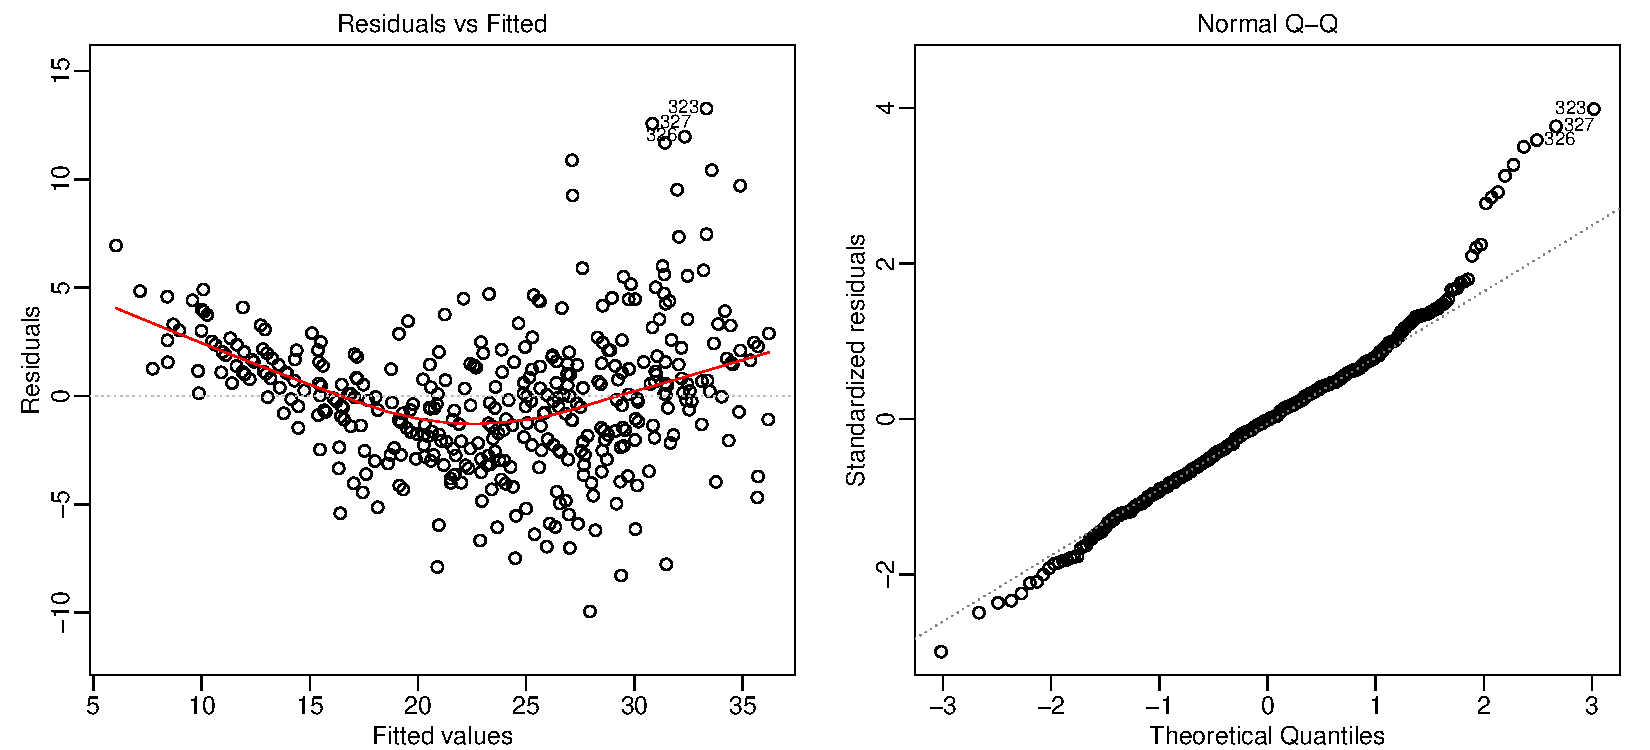
\includegraphics{hw2_fall18_files/figure-latex/unnamed-chunk-17-1.pdf}

\section{\texorpdfstring{Assessment of the model (``Describe the final
model and its accuracy. Include diagnostic plots with particular focus
on the model residuals. Summarize the effects
found.''):}{Assessment of the model (Describe the final model and its accuracy. Include diagnostic plots with particular focus on the model residuals. Summarize the effects found.):}}\label{assessment-of-the-model-describe-the-final-model-and-its-accuracy.-include-diagnostic-plots-with-particular-focus-on-the-model-residuals.-summarize-the-effects-found.}

\section{MPG can be reasonably predicted by using three variables
(weight, year, origin). The model has a good level of accuracy with an
Adjusted Rsquare of 0.816. Diagnostic plot is included in the above
chunk.}\label{mpg-can-be-reasonably-predicted-by-using-three-variables-weight-year-origin.-the-model-has-a-good-level-of-accuracy-with-an-adjusted-rsquare-of-0.816.-diagnostic-plot-is-included-in-the-above-chunk.}

\section{\texorpdfstring{Making Predictions (``Predict the mpg of a car
that is: built in 1983, in US, red, 180 inches long, 8 cylinders, 350
displacement, 260 as horsepower and weighs 4000 pounds. Give a 95\%
CI.'')}{Making Predictions (Predict the mpg of a car that is: built in 1983, in US, red, 180 inches long, 8 cylinders, 350 displacement, 260 as horsepower and weighs 4000 pounds. Give a 95\% CI.)}}\label{making-predictions-predict-the-mpg-of-a-car-that-is-built-in-1983-in-us-red-180-inches-long-8-cylinders-350-displacement-260-as-horsepower-and-weighs-4000-pounds.-give-a-95-ci.}

\begin{Shaded}
\begin{Highlighting}[]
\NormalTok{predicted.mpg <-}\StringTok{ }\NormalTok{data2[}\DecValTok{1}\NormalTok{,]}
\NormalTok{predicted.mpg}\OperatorTok{$}\NormalTok{mpg <-}\StringTok{ }\OtherTok{NA}
\NormalTok{predicted.mpg}\OperatorTok{$}\NormalTok{year <-}\StringTok{ }\DecValTok{83}
\NormalTok{predicted.mpg}\OperatorTok{$}\NormalTok{origin <-}\StringTok{ }\DecValTok{1}
\NormalTok{predicted.mpg}\OperatorTok{$}\NormalTok{cylinders <-}\StringTok{ }\DecValTok{8}
\NormalTok{predicted.mpg}\OperatorTok{$}\NormalTok{displacement <-}\StringTok{ }\DecValTok{350}
\NormalTok{predicted.mpg}\OperatorTok{$}\NormalTok{horsepower <-}\StringTok{ }\DecValTok{260}
\NormalTok{predicted.mpg}\OperatorTok{$}\NormalTok{weight <-}\StringTok{ }\DecValTok{4000}

\NormalTok{predicted.mpg.final.model <-}\StringTok{ }\KeywordTok{predict}\NormalTok{(fit.final, predicted.mpg, }\DataTypeTok{interval=}\StringTok{"confidence"}\NormalTok{, }\DataTypeTok{se.fit=}\OtherTok{TRUE}\NormalTok{) }
\KeywordTok{print}\NormalTok{(predicted.mpg.final.model)}
\end{Highlighting}
\end{Shaded}

\begin{verbatim}
## $fit
##        fit      lwr      upr
## 1 21.96954 21.01736 22.92172
## 
## $se.fit
## [1] 0.4842996
## 
## $df
## [1] 388
## 
## $residual.scale
## [1] 3.347605
\end{verbatim}

\section{fit lwr upr}\label{fit-lwr-upr}

\section{1 21.96954 21.01736 22.92172}\label{section}

\section{\$se.fit}\label{se.fit}

\section{{[}1{]} 0.4842996}\label{section-1}

\section{The predicted MPG for such car is 21.97 (21.02,
22.92)}\label{the-predicted-mpg-for-such-car-is-21.97-21.02-22.92}

\subsection{Problem 3: Lasso}\label{problem-3-lasso}

Crime data continuation: We use a subset of the crime data discussed in
class, but only look at Florida and California. \texttt{crimedata} is
available on Canvas; we show the code to clean here.

\begin{Shaded}
\begin{Highlighting}[]
\NormalTok{cdata <-}\StringTok{ }\KeywordTok{read.csv}\NormalTok{(}\StringTok{"CrimeData_clean.csv"}\NormalTok{, }\DataTypeTok{stringsAsFactors =}\NormalTok{ F, }\DataTypeTok{na.strings =} \KeywordTok{c}\NormalTok{(}\StringTok{"?"}\NormalTok{)) ## load crime data file}
\NormalTok{cdata <-}\StringTok{ }\NormalTok{dplyr}\OperatorTok{::}\KeywordTok{filter}\NormalTok{(cdata, state }\OperatorTok\StringTok{ }\KeywordTok{c}\NormalTok{(}\StringTok{"FL"}\NormalTok{, }\StringTok{"CA"}\NormalTok{)) ## filter data for Florida and California }
\KeywordTok{dim}\NormalTok{(cdata)}
\end{Highlighting}
\end{Shaded}

\begin{verbatim}
## [1] 368  99
\end{verbatim}

Our goal is to find the factors which relate to violent crime. This
variable is included in crime as \texttt{crime\$violentcrimes.perpop}.

Use LASSO to choose a reasonable, small model. Fit an OLS model with the
variables obtained. The final model should only include variables with
p-values \textless{} 0.05. Note: you may choose to use lambda 1st or
lambda min to answer the following questions where apply.

\begin{enumerate}
\def\labelenumi{\arabic{enumi}.}
\tightlist
\item
  What is the model reported by LASSO?
\end{enumerate}

\begin{Shaded}
\begin{Highlighting}[]
\NormalTok{Yvar <-}\StringTok{ }\NormalTok{cdata[,}\DecValTok{99}\NormalTok{] ## extracting Y}
\NormalTok{Xvar <-}\StringTok{ }\KeywordTok{model.matrix}\NormalTok{(violentcrimes.perpop}\OperatorTok{~}\NormalTok{., }\DataTypeTok{data =}\NormalTok{ cdata)[,}\DecValTok{3}\OperatorTok{:}\DecValTok{99}\NormalTok{] ## extracting X }
\KeywordTok{colnames}\NormalTok{(Xvar)}
\end{Highlighting}
\end{Shaded}

\begin{verbatim}
##  [1] "population"                      "household.size"                 
##  [3] "race.pctblack"                   "race.pctwhite"                  
##  [5] "race.pctasian"                   "race.pcthisp"                   
##  [7] "age.pct12to21"                   "age.pct12to29"                  
##  [9] "age.pct16to24"                   "age.pct65up"                    
## [11] "pct.urban"                       "med.income"                     
## [13] "pct.wage.inc"                    "pct.farmself.inc"               
## [15] "pct.inv.inc"                     "pct.socsec.inc"                 
## [17] "pct.pubasst.inc"                 "pct.retire"                     
## [19] "med.family.inc"                  "percap.inc"                     
## [21] "white.percap"                    "black.percap"                   
## [23] "indian.percap"                   "asian.percap"                   
## [25] "hisp.percap"                     "pct.pop.underpov"               
## [27] "pct.less9thgrade"                "pct.not.hsgrad"                 
## [29] "pct.bs.ormore"                   "pct.unemployed"                 
## [31] "pct.employed"                    "pct.employed.manuf"             
## [33] "pct.employed.profserv"           "pct.occup.manuf"                
## [35] "pct.occup.mgmtprof"              "male.pct.divorce"               
## [37] "male.pct.nvrmarried"             "female.pct.divorce"             
## [39] "total.pct.divorce"               "ave.people.per.fam"             
## [41] "pct.fam2parents"                 "pct.kids2parents"               
## [43] "pct.youngkids2parents"           "pct.teens2parents"              
## [45] "pct.workmom.youngkids"           "pct.workmom"                    
## [47] "num.kids.nvrmarried"             "pct.kids.nvrmarried"            
## [49] "num.immig"                       "pct.immig.recent"               
## [51] "pct.immig.recent5"               "pct.immig.recent8"              
## [53] "pct.immig.recent10"              "pct.pop.immig"                  
## [55] "pct.pop.immig5"                  "pct.pop.immig8"                 
## [57] "pct.pop.immig10"                 "pct.english.only"               
## [59] "pct.no.english.well"             "pct.fam.hh.large"               
## [61] "pct.occup.hh.large"              "ave.people.per.hh"              
## [63] "ave.people.per.ownoccup.hh"      "ave.people.per.rented.hh"       
## [65] "pct.people.ownoccup.hh"          "pct.people.dense.hh"            
## [67] "pct.hh.less3br"                  "med.num.br"                     
## [69] "pct.house.occup"                 "pct.house.ownoccup"             
## [71] "pct.house.vacant"                "pct.house.vacant.6moplus"       
## [73] "med.yr.house.built"              "pct.house.nophone"              
## [75] "pct.house.no.plumb"              "value.ownoccup.house.lowquart"  
## [77] "value.ownoccup.med"              "value.ownoccup.highquart"       
## [79] "ownoccup.qrange"                 "rent.lowquart"                  
## [81] "rent.med"                        "rent.highquart"                 
## [83] "rent.qrange"                     "med.rent"                       
## [85] "med.rent.aspct.hhinc"            "med.owncost.aspct.hhinc.wmort"  
## [87] "med.owncost.as.pct.hhinc.womort" "num.in.shelters"                
## [89] "num.homeless"                    "pct.foreignborn"                
## [91] "pct.born.samestate"              "pct.samehouse1985"              
## [93] "pct.samecity1985"                "pct.samestate1985"              
## [95] "land.area"                       "pop.density"                    
## [97] "pct.use.publictransit"
\end{verbatim}

\begin{Shaded}
\begin{Highlighting}[]
\NormalTok{lass <-}\StringTok{ }\KeywordTok{glmnet}\NormalTok{(Xvar, Yvar, }\DataTypeTok{alpha =} \DecValTok{1}\NormalTok{) }
\KeywordTok{str}\NormalTok{(lass)}
\end{Highlighting}
\end{Shaded}

\begin{verbatim}
## List of 12
##  $ a0       : Named num [1:100] 896 904 1038 1160 1272 ...
##   ..- attr(*, "names")= chr [1:100] "s0" "s1" "s2" "s3" ...
##  $ beta     :Formal class 'dgCMatrix' [package "Matrix"] with 6 slots
##   .. ..@ i       : int [1:4484] 41 47 41 47 41 47 41 47 41 47 ...
##   .. ..@ p       : int [1:101] 0 0 2 4 6 8 10 12 15 18 ...
##   .. ..@ Dim     : int [1:2] 97 100
##   .. ..@ Dimnames:List of 2
##   .. .. ..$ : chr [1:97] "population" "household.size" "race.pctblack" "race.pctwhite" ...
##   .. .. ..$ : chr [1:100] "s0" "s1" "s2" "s3" ...
##   .. ..@ x       : num [1:4484] -0.872 14.625 -3.277 23.407 -5.467 ...
##   .. ..@ factors : list()
##  $ df       : int [1:100] 0 2 2 2 2 2 2 3 3 3 ...
##  $ dim      : int [1:2] 97 100
##  $ lambda   : num [1:100] 510 465 423 386 352 ...
##  $ dev.ratio: num [1:100] 0 0.104 0.198 0.276 0.34 ...
##  $ nulldev  : num 1.62e+08
##  $ npasses  : int 6877
##  $ jerr     : int 0
##  $ offset   : logi FALSE
##  $ call     : language glmnet(x = Xvar, y = Yvar, alpha = 1)
##  $ nobs     : int 368
##  - attr(*, "class")= chr [1:2] "elnet" "glmnet"
\end{verbatim}

\begin{Shaded}
\begin{Highlighting}[]
\KeywordTok{plot}\NormalTok{(lass) ## plot LASSO graph}
\end{Highlighting}
\end{Shaded}

\includegraphics{hw2_fall18_files/figure-latex/unnamed-chunk-21-1.pdf}

\begin{Shaded}
\begin{Highlighting}[]
\NormalTok{crime <-}\StringTok{ }\KeywordTok{cv.glmnet}\NormalTok{(Xvar, Yvar, }\DataTypeTok{alpha=}\DecValTok{1}\NormalTok{, }\DataTypeTok{nfolds=}\DecValTok{10}\NormalTok{) }\CommentTok{#cross validation }
\NormalTok{crime}\OperatorTok{$}\NormalTok{cvm }\CommentTok{#  mean cv error }
\end{Highlighting}
\end{Shaded}

\begin{verbatim}
##  [1] 439692.9 398299.2 357199.5 322667.8 294035.4 270295.7 250577.0
##  [8] 234016.9 219833.0 207516.5 197098.1 188461.4 181314.6 175404.1
## [15] 170523.5 166380.0 162162.6 159000.3 156965.1 155708.4 155123.5
## [22] 155161.6 155675.0 156482.5 157395.4 158467.6 159151.4 159359.6
## [29] 159191.6 159220.0 159267.5 159486.7 159808.1 160293.3 160979.1
## [36] 161911.1 162990.0 164104.9 165206.0 166197.0 166838.5 167342.2
## [43] 167595.4 167804.8 167888.2 167343.4 165915.8 164861.2 163615.8
## [50] 162295.2 161390.4 160560.9 160343.4 160426.3 161477.0 162499.0
## [57] 163553.6 164527.8 165350.7 165264.6 164863.1 164906.3 164923.7
## [64] 165025.6 165019.5 165183.8 165700.1 166364.6 166951.4 167418.2
## [71] 167811.4 168313.3 168753.5 169378.5 170166.7 170898.5 171827.2
## [78] 172640.3 173484.1 174176.5 175066.3 175845.3 176667.6 177493.7
## [85] 178294.5 179119.1 179922.1 180565.8 181280.7 181846.9
\end{verbatim}

\begin{Shaded}
\begin{Highlighting}[]
\NormalTok{crime}\OperatorTok{$}\NormalTok{lambda.min }\CommentTok{#  min point among all the cvm}
\end{Highlighting}
\end{Shaded}

\begin{verbatim}
## [1] 79.336
\end{verbatim}

\begin{Shaded}
\begin{Highlighting}[]
\NormalTok{crime}\OperatorTok{$}\NormalTok{nzero }\CommentTok{# non-zero coeff's }
\end{Highlighting}
\end{Shaded}

\begin{verbatim}
##  s0  s1  s2  s3  s4  s5  s6  s7  s8  s9 s10 s11 s12 s13 s14 s15 s16 s17 
##   0   2   2   2   2   2   2   3   3   3   3   3   3   3   3   3   3   3 
## s18 s19 s20 s21 s22 s23 s24 s25 s26 s27 s28 s29 s30 s31 s32 s33 s34 s35 
##   4   4   4   5   5   6   6  10  11  11  12  14  15  15  15  16  18  19 
## s36 s37 s38 s39 s40 s41 s42 s43 s44 s45 s46 s47 s48 s49 s50 s51 s52 s53 
##  21  23  22  24  24  27  30  32  33  35  38  43  43  43  46  45  44  44 
## s54 s55 s56 s57 s58 s59 s60 s61 s62 s63 s64 s65 s66 s67 s68 s69 s70 s71 
##  45  48  50  54  56  55  58  61  64  65  70  69  70  73  74  75  75  75 
## s72 s73 s74 s75 s76 s77 s78 s79 s80 s81 s82 s83 s84 s85 s86 s87 s88 s89 
##  77  77  81  83  85  88  89  89  89  90  88  90  90  91  91  90  91  92
\end{verbatim}

\begin{Shaded}
\begin{Highlighting}[]
\KeywordTok{plot}\NormalTok{(crime)}
\end{Highlighting}
\end{Shaded}

\includegraphics{hw2_fall18_files/figure-latex/unnamed-chunk-22-1.pdf}
2. What is the model after running OLS?

\begin{Shaded}
\begin{Highlighting}[]
\NormalTok{cof <-}\StringTok{ }\KeywordTok{coef}\NormalTok{(crime, }\DataTypeTok{s=}\StringTok{"lambda.1se"}\NormalTok{) ## lambda 1se}
\NormalTok{cof <-}\StringTok{ }\NormalTok{cof[}\KeywordTok{which}\NormalTok{(cof }\OperatorTok{!=}\DecValTok{0}\NormalTok{),] }\CommentTok{# to get  non-zero coefficients }
\NormalTok{var <-}\StringTok{ }\KeywordTok{rownames}\NormalTok{(}\KeywordTok{as.matrix}\NormalTok{(cof)) }
\NormalTok{input <-}\StringTok{ }\KeywordTok{as.formula}\NormalTok{(}\KeywordTok{paste}\NormalTok{(}\StringTok{"violentcrimes.perpop"}\NormalTok{, }\StringTok{"~"}\NormalTok{, }\KeywordTok{paste}\NormalTok{(var[}\OperatorTok{-}\DecValTok{1}\NormalTok{], }\DataTypeTok{collapse =} \StringTok{"+"}\NormalTok{))) }\CommentTok{# prepare input}
\end{Highlighting}
\end{Shaded}

\begin{Shaded}
\begin{Highlighting}[]
\NormalTok{lmse <-}\StringTok{ }\KeywordTok{lm}\NormalTok{(input, }\DataTypeTok{data=}\NormalTok{cdata)}
\NormalTok{output <-}\StringTok{ }\KeywordTok{coef}\NormalTok{(lmse) }\CommentTok{# output lm estimates}
\KeywordTok{summary}\NormalTok{(lmse)}
\end{Highlighting}
\end{Shaded}

\begin{verbatim}
## 
## Call:
## lm(formula = input, data = cdata)
## 
## Residuals:
##      Min       1Q   Median       3Q      Max 
## -1115.29  -210.52   -37.48   155.25  1911.97 
## 
## Coefficients:
##                     Estimate Std. Error t value Pr(>|t|)    
## (Intercept)         2012.949    266.282   7.559 3.32e-13 ***
## race.pctblack         13.956      2.742   5.089 5.78e-07 ***
## pct.kids2parents     -22.678      3.371  -6.728 6.70e-11 ***
## pct.kids.nvrmarried   94.953     12.269   7.739 9.95e-14 ***
## ---
## Signif. codes:  0 '***' 0.001 '**' 0.01 '*' 0.05 '.' 0.1 ' ' 1
## 
## Residual standard error: 378.3 on 364 degrees of freedom
## Multiple R-squared:  0.6791, Adjusted R-squared:  0.6765 
## F-statistic: 256.8 on 3 and 364 DF,  p-value: < 2.2e-16
\end{verbatim}

\begin{Shaded}
\begin{Highlighting}[]
\NormalTok{comp <-}\StringTok{ }\KeywordTok{data.frame}\NormalTok{(cof, output )}
\KeywordTok{names}\NormalTok{(comp) <-}\StringTok{ }\KeywordTok{c}\NormalTok{(}\StringTok{"estimates from LASSO"}\NormalTok{, }\StringTok{"lm estimates"}\NormalTok{)}
\NormalTok{comp}
\end{Highlighting}
\end{Shaded}

\begin{verbatim}
##                     estimates from LASSO lm estimates
## (Intercept)                  1768.766553   2012.94869
## race.pctblack                   6.733932     13.95606
## pct.kids2parents              -17.309554    -22.67806
## pct.kids.nvrmarried            75.092585     94.95302
\end{verbatim}

\begin{enumerate}
\def\labelenumi{\arabic{enumi}.}
\setcounter{enumi}{2}
\tightlist
\item
  What is your final model, after excluding high p-value variables?
\end{enumerate}

Now, instead of Lasso, we want to consider how changing the value of
alpha (i.e.~mixing between Lasso and Ridge) will affect the model.
Cross-validate between alpha and lambda, instead of just lambda. Note
that the final model may have variables with p-values higher than 0.05;
this is because we are optimizing for accuracy rather than
parsimoniousness.

\begin{enumerate}
\def\labelenumi{\arabic{enumi}.}
\tightlist
\item
  What is your final elastic net model? What were the alpha and lambda
  values? What is the prediction error?
\end{enumerate}

\begin{Shaded}
\begin{Highlighting}[]
\NormalTok{fit2 <-}\StringTok{ }\KeywordTok{glmnet}\NormalTok{(Xvar, Yvar, }\DataTypeTok{alpha=}\NormalTok{.}\DecValTok{99}\NormalTok{)}
\NormalTok{fit2.cv <-}\StringTok{ }\KeywordTok{cv.glmnet}\NormalTok{(Xvar, Yvar, }\DataTypeTok{alpha=}\NormalTok{.}\DecValTok{99}\NormalTok{, }\DataTypeTok{nfolds=}\DecValTok{10}\NormalTok{)}
\NormalTok{fit2.cv}\OperatorTok{$}\NormalTok{lambda.1se}
\end{Highlighting}
\end{Shaded}

\begin{verbatim}
## [1] 140.0423
\end{verbatim}

\begin{Shaded}
\begin{Highlighting}[]
\KeywordTok{plot}\NormalTok{(fit2.cv)}
\end{Highlighting}
\end{Shaded}

\includegraphics{hw2_fall18_files/figure-latex/unnamed-chunk-26-1.pdf}
2. Use the elastic net variables in an OLS model. What is the equation,
and what is the prediction error.

\begin{Shaded}
\begin{Highlighting}[]
\NormalTok{cof2 <-}\StringTok{ }\KeywordTok{coef}\NormalTok{(fit2.cv, }\DataTypeTok{s=}\StringTok{"lambda.1se"}\NormalTok{) }
\NormalTok{cof2 <-}\StringTok{ }\NormalTok{cof2[}\KeywordTok{which}\NormalTok{(cof2 }\OperatorTok{!=}\DecValTok{0}\NormalTok{),] ##  non-zero coefficients}
\NormalTok{var2 <-}\StringTok{ }\KeywordTok{rownames}\NormalTok{(}\KeywordTok{as.matrix}\NormalTok{(cof2)) ## output names}
\NormalTok{input2 <-}\StringTok{ }\KeywordTok{as.formula}\NormalTok{(}\KeywordTok{paste}\NormalTok{(}\StringTok{"violentcrimes.perpop"}\NormalTok{, }\StringTok{"~"}\NormalTok{, }\KeywordTok{paste}\NormalTok{(var2[}\OperatorTok{-}\DecValTok{1}\NormalTok{], }\DataTypeTok{collapse =} \StringTok{"+"}\NormalTok{))) }\CommentTok{# prepare input}
\NormalTok{lm2 <-}\StringTok{ }\KeywordTok{lm}\NormalTok{(input2, }\DataTypeTok{data=}\NormalTok{cdata)}
\NormalTok{output2 <-}\StringTok{ }\KeywordTok{coef}\NormalTok{(lm2) }\CommentTok{# output lm estimates}
\KeywordTok{summary}\NormalTok{(lm2)}
\end{Highlighting}
\end{Shaded}

\begin{verbatim}
## 
## Call:
## lm(formula = input2, data = cdata)
## 
## Residuals:
##      Min       1Q   Median       3Q      Max 
## -1115.29  -210.52   -37.48   155.25  1911.97 
## 
## Coefficients:
##                     Estimate Std. Error t value Pr(>|t|)    
## (Intercept)         2012.949    266.282   7.559 3.32e-13 ***
## race.pctblack         13.956      2.742   5.089 5.78e-07 ***
## pct.kids2parents     -22.678      3.371  -6.728 6.70e-11 ***
## pct.kids.nvrmarried   94.953     12.269   7.739 9.95e-14 ***
## ---
## Signif. codes:  0 '***' 0.001 '**' 0.01 '*' 0.05 '.' 0.1 ' ' 1
## 
## Residual standard error: 378.3 on 364 degrees of freedom
## Multiple R-squared:  0.6791, Adjusted R-squared:  0.6765 
## F-statistic: 256.8 on 3 and 364 DF,  p-value: < 2.2e-16
\end{verbatim}

\begin{enumerate}
\def\labelenumi{\arabic{enumi}.}
\setcounter{enumi}{2}
\tightlist
\item
  Summarize your findings, with particular focus on the difference
  between the two equations.
\end{enumerate}

\begin{Shaded}
\begin{Highlighting}[]
\NormalTok{comp2 <-}\StringTok{ }\KeywordTok{data.frame}\NormalTok{(cof2, output2 )}
\KeywordTok{names}\NormalTok{(comp2) <-}\StringTok{ }\KeywordTok{c}\NormalTok{(}\StringTok{"estimates from Elastic Net"}\NormalTok{, }\StringTok{"lm estimates"}\NormalTok{)}
\NormalTok{comp2}
\end{Highlighting}
\end{Shaded}

\begin{verbatim}
##                     estimates from Elastic Net lm estimates
## (Intercept)                        1767.966054   2012.94869
## race.pctblack                         6.760708     13.95606
## pct.kids2parents                    -17.291978    -22.67806
## pct.kids.nvrmarried                  74.920146     94.95302
\end{verbatim}


\end{document}
